%%%%%%%%%%%%%%%%%%%%%%%%%%%%%%%%%%%%%%%%%%%
%%% DOCUMENT PREAMBLE %%%
\documentclass[12pt]{report}

%\usepackage{natbib}
\usepackage{subfigure}
\usepackage{amsmath,amssymb,array,biblatex,bm,caption,fancyhdr,float,graphicx,indentfirst,parskip,url,vmargin}
\graphicspath{{images/}}
\addbibresource{project.bib}
\captionsetup[figure]{labelsep=period}
\begin{document}
\setlength{\parindent}{1em}
\vspace*{0.25cm}
\hrulefill
\thispagestyle{empty}
\begin{center}
    \begin{large}
        \sc{UM--SJTU Joint Institute
        \vspace{0.3em}\\
        Numerical solution of Newton’s equations of motion
        \vspace{0.3em}\\
        VP160 Project
        \vspace{0.3em}\\}
    \end{large}
    \hrulefill
    \vspace*{5cm}\\
    \begin{large}
        \sc{Project Group 22}
    \end{large}
\end{center}
\vfill
\begin{large}
    \sc{Group Members:}
\end{large}
\begin{table}[h!]
    \flushleft
    \begin{tabular}{ll}
        Cai Yiteng \hspace*{3em}&518370910007\hspace*{3em}\\
        Fang Han \hspace*{3em}&518370910009\hspace*{3em}\\
        Liu Yihua \hspace*{3em}&518021910998\hspace*{3em}\\
        Li Xiwen \hspace*{3em}&518021910415\hspace*{3em}\\
        \\
        Date: \today
    \end{tabular}
\end{table}

\textit{We state that each of us has contributed equally to this project.}\\

Signature:\underline{\makebox[25em]{                                         }}
\hfill
\clearpage
\renewcommand{\thesection}{\arabic{section}}
\section{Introduction}
While studying the Newton's dynamic, a basic thing we need to do is to solve the equation of the motion of a particle. According to the Newton's Second Law, an equation of motion can be written as
\begin{equation}
    \frac{d^2r}{dt^2}=F(v,r,t)
\end{equation}
If the equation can be solved, we can easily predict the place and movement of a particle at a specific time. However, if the equation is too complex to solve, in order to predict its motion, we need to do some approximation. Two classic models of approximation are the Euler's Method and Heun's Method.
\subsection{Euler's Method}
Firstly, we will discuss about Euler's Method. We all know Taylor's expansion of a function can be written as
\begin{equation}
    f(x)=f(x_{0})+f'(x_{0})(x-x_{0})+\frac{1}{2!}f''(x_{0})(x-x_{0})+...
\end{equation}
For an x near $x_{0}$, we can basically approximate that
\begin{equation}
    f(x)\approx f(x_{0})+f'(x_{0})(x-x_{0})
\end{equation}
The Euler's Method is based on that idea. We denote $x^*$ as the approximate value of x, so do other physical quantities. Then we can have a recursive equation like that, in the 1-D case motion, for given values of $x_{0}$, $v_{0}$ at a specific moment, we can write the approximation value after i$\Delta t$
\begin{equation}
    x_{0}^*=x_{0}
\end{equation}
\begin{equation}
    v_{x,i+1}^*=v_{x,i}^*+\frac{F_{x}(v_{x,i}^*,x_{i}^*,t_{i})}{m}\Delta t
\end{equation}
\begin{equation}
    x_{x,0}^*=x_{0}
\end{equation}
\begin{equation}
    x_{i+1}^*=x_{i}^*+v_{x,i}\Delta t
\end{equation}
\begin{equation}
    t_{i+1}=i\Delta t
\end{equation}
Starting with t=1, and we can calculate the approximation value of $x_{t}$, $v_{t}$ at a specific moment t by this algorithm.
\subsection{Heun's Method}
The Heun's Method is actually a revise of the Euler's Method. Since the f'($x_{0}$) cannot always approximate the next value very well, we decide to revise it by replacing $k_{1}$ with $\frac{1}{2}(K_{1}+k_{2}$, where $K_{2}$ is the approximate slope at the right end. In fact, we always approximate $k_{2}$ by applying the Euler's Method. We denote the slope at $x_{i}$ as $G(f_{i}^*,t_{i})$. Thus, we can calculate the result by
\begin{equation}
    f_{0}^*=f_{0}
\end{equation}
\begin{equation}
    k_{1}=G(f_{i}^*,t_{i})
\end{equation}
\begin{equation}
    k_{2}=G(f_{i}^*+k_{1}\Delta t,t_{i}+\Delta t)
\end{equation}
\begin{equation}
    f_{i+1}^*=f_{i}^*+\frac{1}{2}(k_{1}+k_{2})\Delta t
\end{equation}
Applying Heun's Method, we can obtain a better approximation of the motion. We will see it in our next discussion.
\clearpage
\section{Projectile motion with air drag}
First consider the problem of a 2D projectile of mass m = 1 kg moving with a linear drag, moving close to the Earth’s surface. The equation of motion in this problem is
\begin{equation}
    \Ddot{r}=-g-\kappa v
\end{equation}
where $\kappa$= k/m and k is the drag coefficient. We assume that the projectile starts out at the origin with velocity $v_{0}$ = 90 m/s at an angle $\alpha$ to the horizontal.
\subsection{Linear Drag}
To find the recursive equations for velocity and position of the projectile, we first want to consider the function of force about three variables velocity $v_i^*$, position $x_i^*$, and time $t_i$. We expand Eq.1 to 2D motion on both $x$ and $y$ directions,
\begin{equation}
    F_x=m\Ddot{x}=-m\kappa v_x^*
\end{equation}

Substituting $F_x$ into the general recursive equation
\begin{equation}
    v_{x,i+1}^*=v_{x,i}^*+\dfrac{F_x(v_i^*,x_i^*,t_i)}{m}\Delta t
\end{equation}
we have
\begin{equation}
    v_{x,i+1}^*=v_{x,i}^*-\kappa v_{x,i}^*\Delta t
\end{equation}

Doing the substitution again for $x$ position,
\begin{equation}
    x_{i+1}^*=x_i^*+v_{x,i}^*\Delta t
\end{equation}

Similarly, for $y$ component,
\begin{equation}
    v_{y,i+1}=v_{y,i}-(g+\kappa v_{y,i}^*)\Delta t
\end{equation}
and
\begin{equation}
    y_{i+1}^*=y_i^*+v_{y,i}^*\Delta t
\end{equation}

Based on the recursive equations for velocity and position of the projectile, we want to examine the sensitivity of the numerical results to the choice of the step $\Delta t$ by researching on the difference between the analytical results and the numerical results, so we first consider the analytical results. We set the initial conditions $t=0$, $v_x=v_0\cos{\alpha}$, $v_y=v_0\sin{\alpha}$, and $x=y=0$. From Eq.1 we derive two differential equations of the motion of the object
\begin{equation}
    -\kappa v_x=\dot{v_x}
\end{equation}
\begin{equation}
    -g-\kappa v_y=\dot{v_y}
\end{equation}

Solving Eq.8 and Eq.9 together, we have the equations of the velocity
\begin{equation}
    v_x=v_0\cos{\alpha}e^{-\kappa t}
\end{equation}
\begin{equation}
    v_y=(\dfrac{g}{\kappa}+v_0\sin{\alpha})e^{-\kappa t}-\dfrac{g}{\kappa}
\end{equation}

Using the initial conditions of positions to integrate Eq.10 and Eq.11, we have the displacement on both $x$ and $y$ directions
\begin{equation}
    x=\dfrac{v_0\cos{\alpha}}{\kappa}(1-e^{-\kappa t})
\end{equation}
\begin{equation}
    y=(\dfrac{g}{\kappa^2}+\dfrac{v_0\sin{\alpha}}{\kappa})(1-e^{-\kappa t})-\dfrac{gt}{\kappa}
\end{equation}

By choosing $\Delta t=0.001$  s, 0.0001 s, 0.00001 s, we apply a discrete algorithm to the recursive equations. By referring to the measurement data of the gravitational acceleration, we have $g=9.7964\ \rm{m/s^2}$. By assumption, the drag coefficient $\kappa=0.5$. Assuming the initial velocity is $v_0=10 \rm{m/s}$, the angle $\alpha$ to the horizontal is $45^\circ$ and the time $t=1$ s, we have the initial velocity in the direction of x and y $v_{x0}=v_{y0}=7.0711$ m/s. Analytically, the result is $x=5.5645$ m and $y=1.3900$ m. By numerical approximation, the three position coordinates are $x_1=5.5656$ m, $x_2=5.5646$ m, $x_3=5.5645$ m, $y_1=1.3941$ m, $y_2=1.3904$ m, $y_3=1.3901$ m, respectively.
\begin{figure}[H]
    \centering
    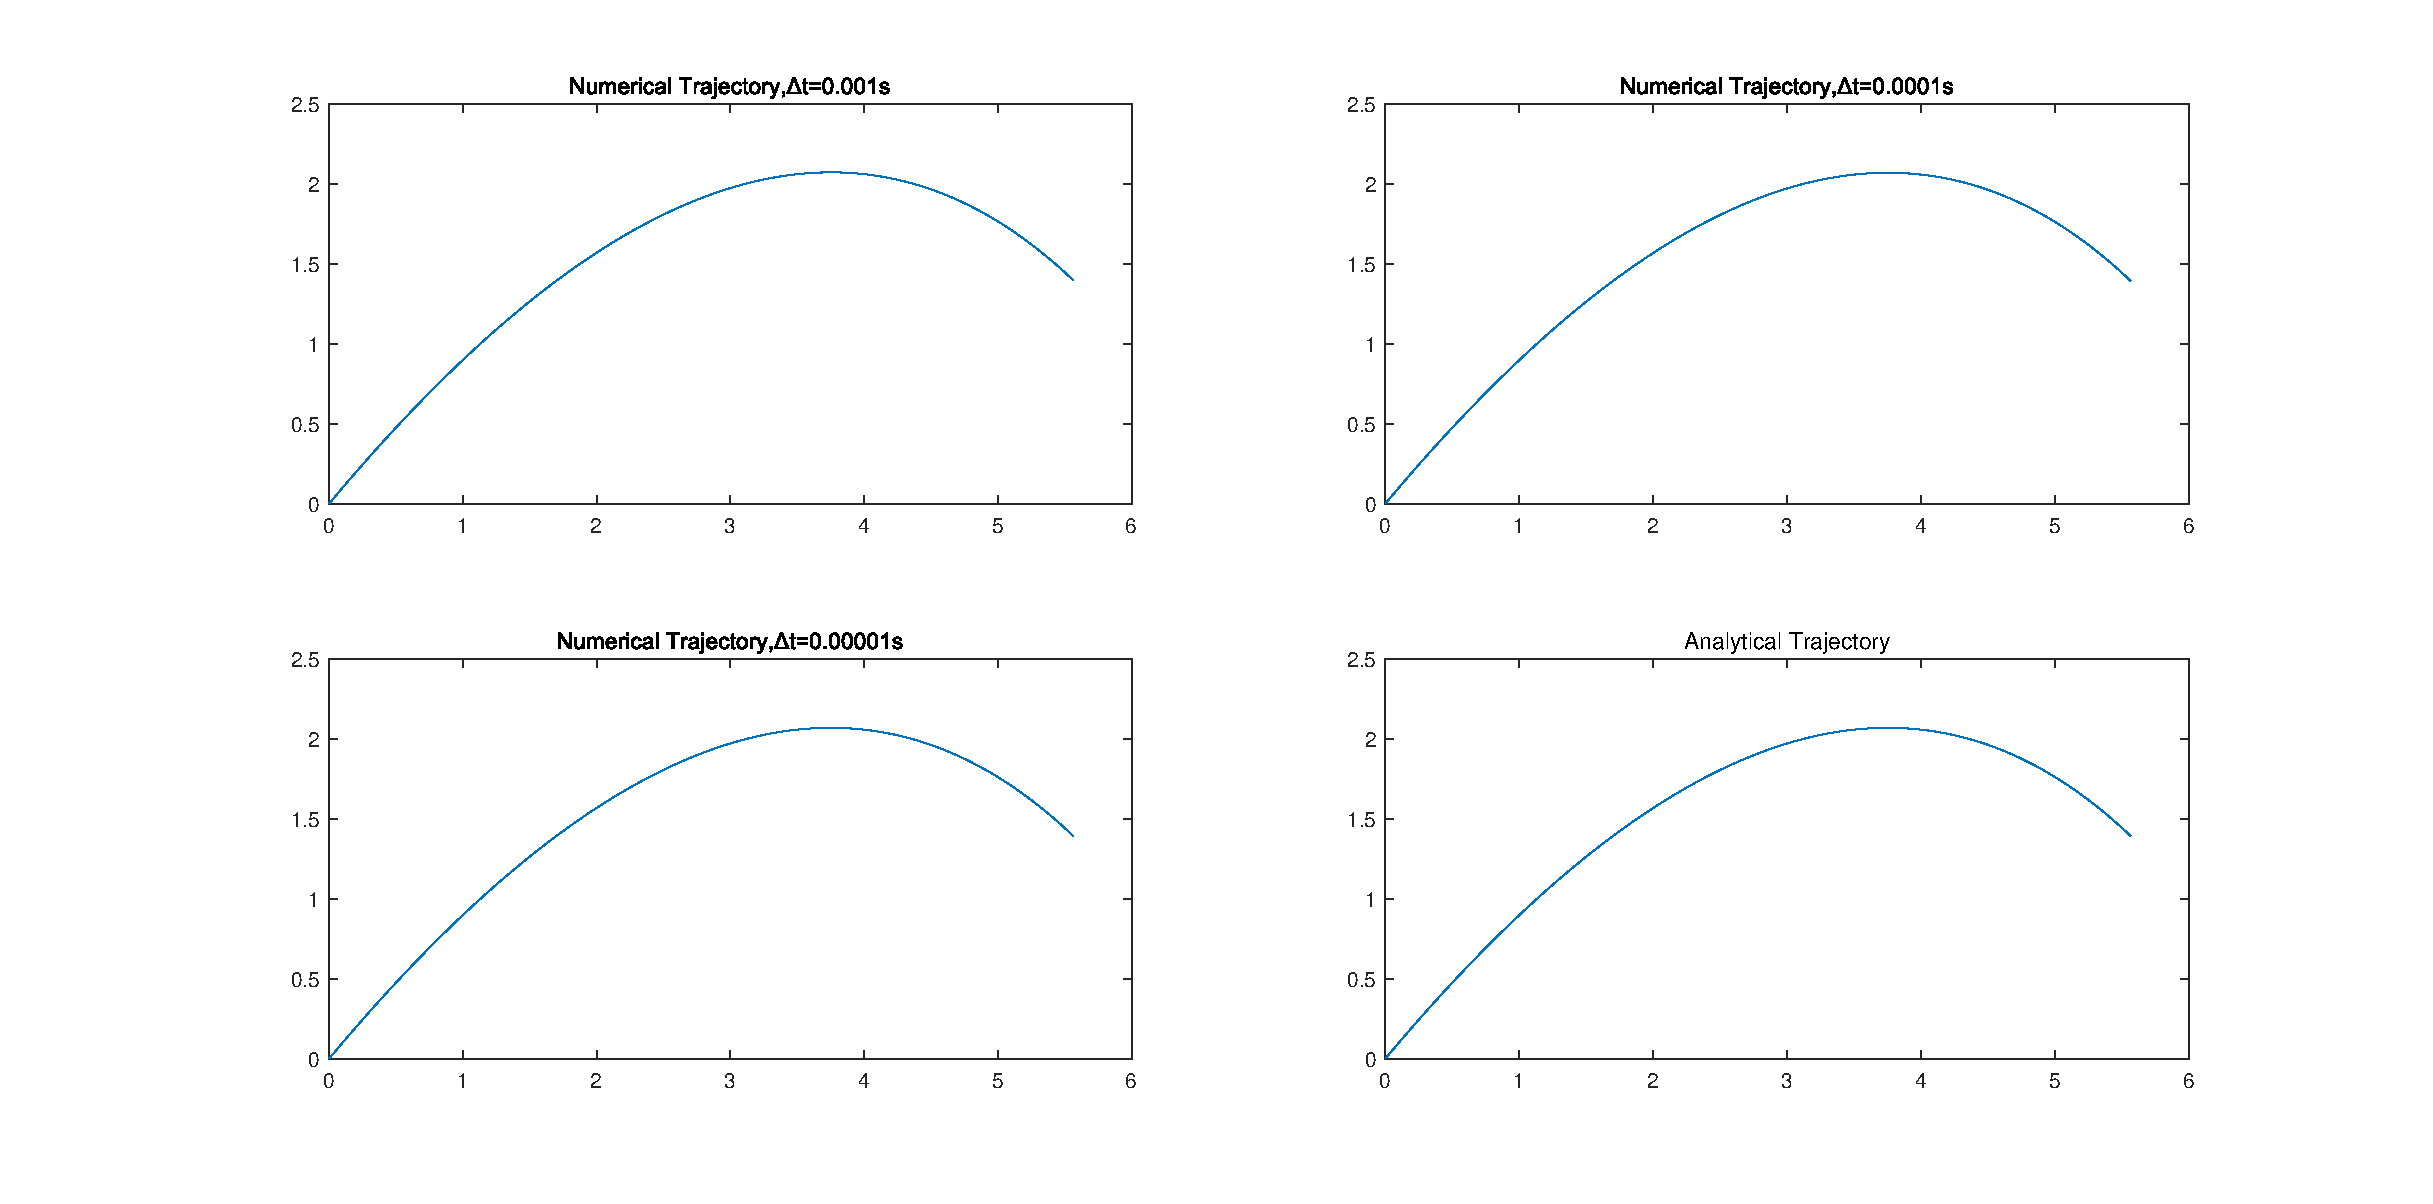
\includegraphics[width=1\linewidth]{2-1-1.eps}
    \caption{Trajectories for linear drag}
\end{figure}
\begin{figure}[H]
    \centering
    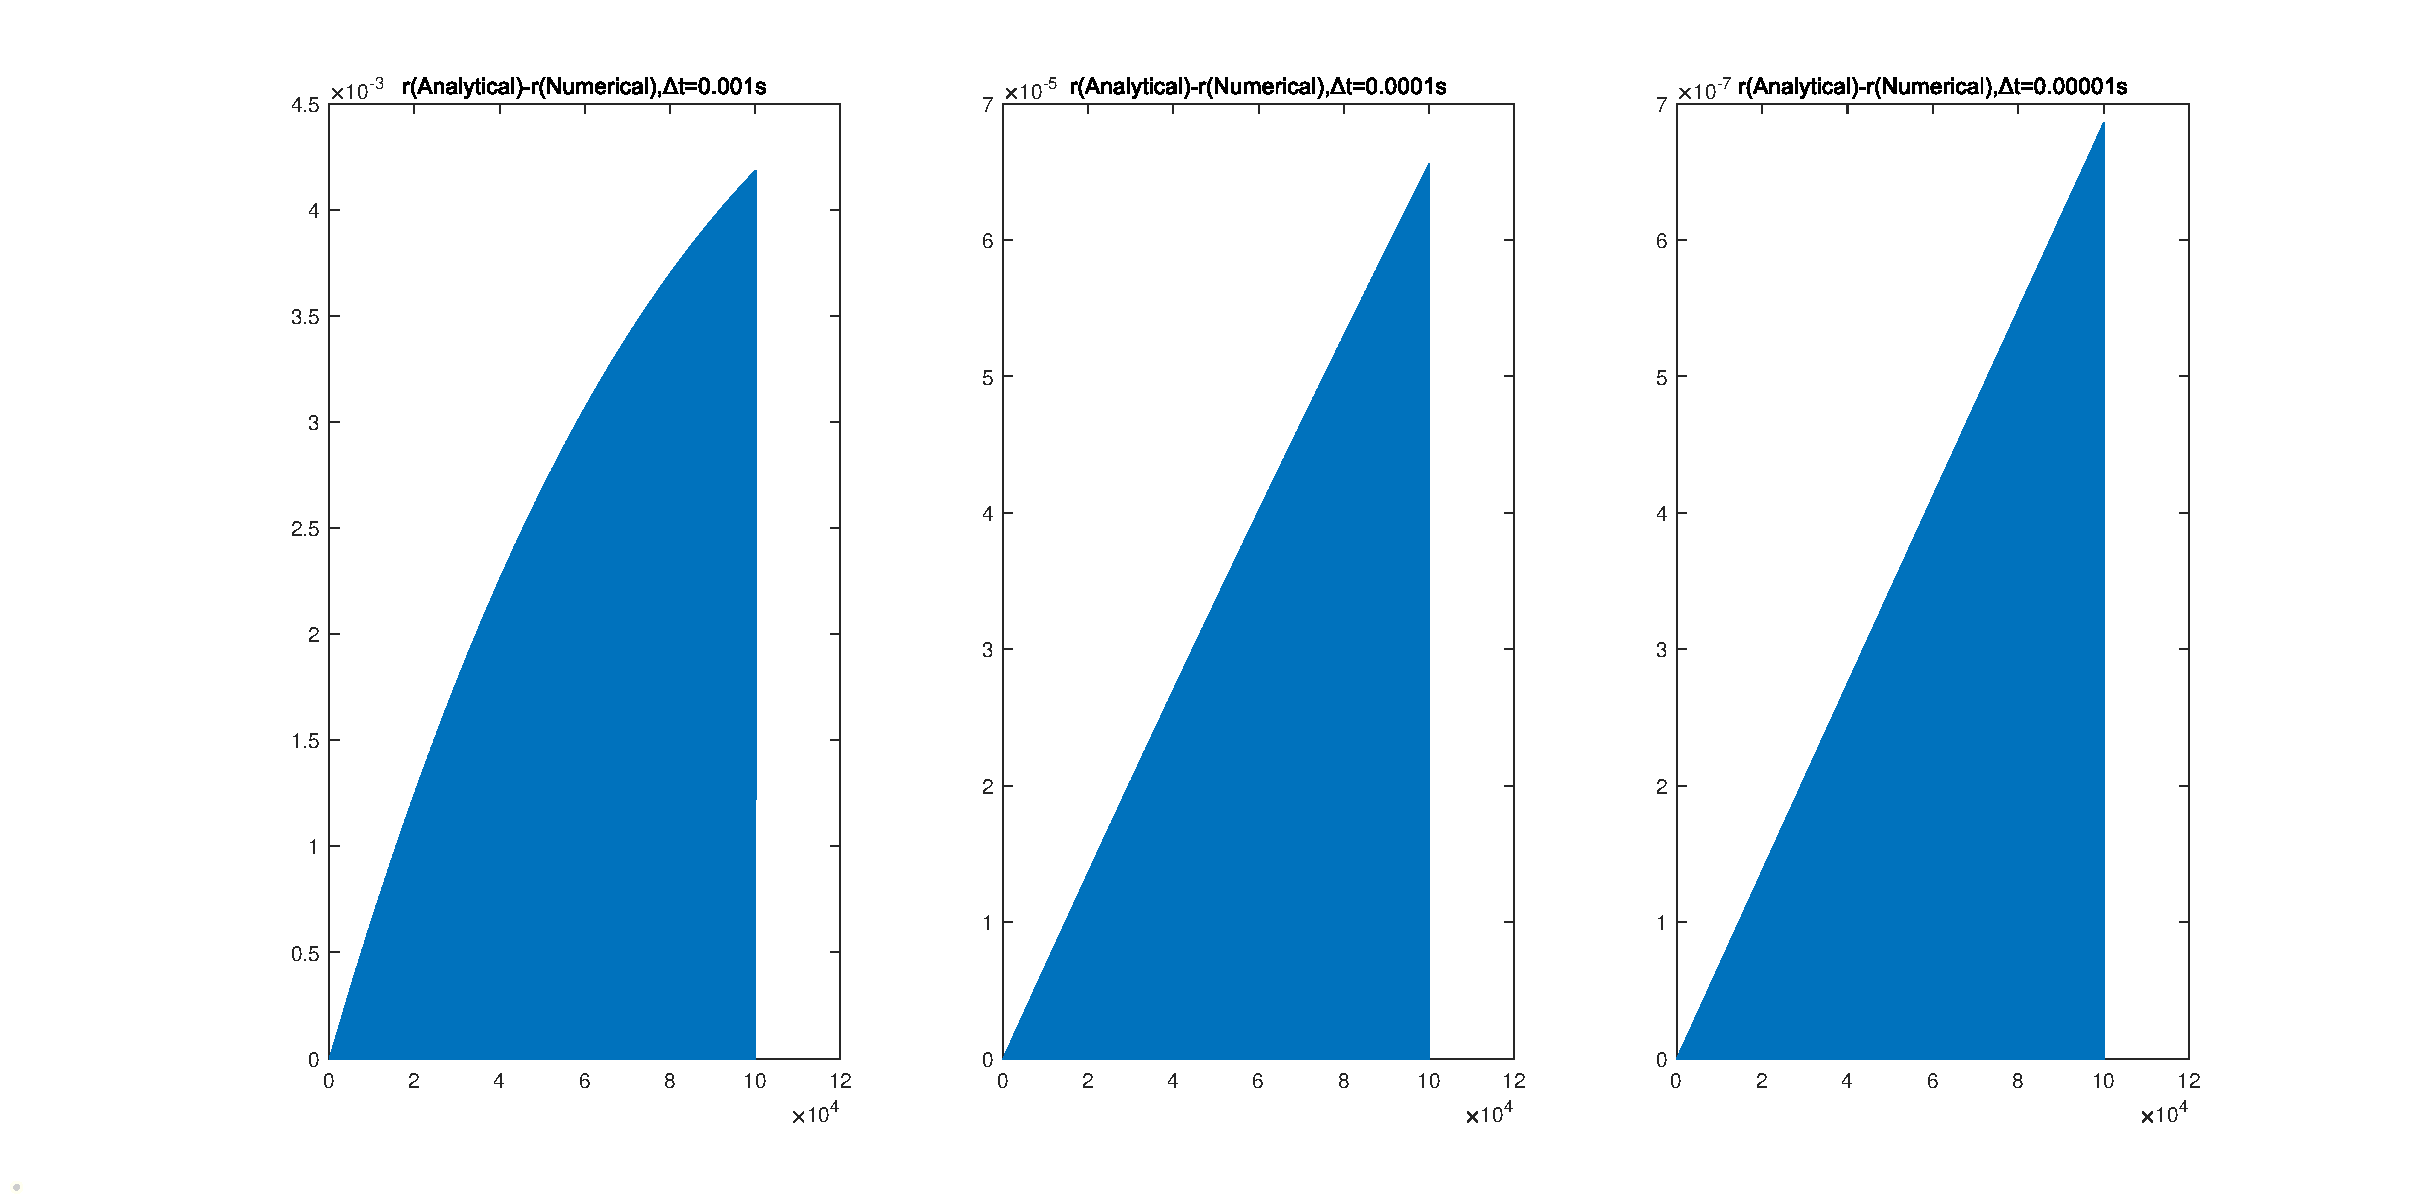
\includegraphics[width=1\linewidth]{2-1-2.eps}
    \caption{$\left| \rm{\bm{r}_{analytical}-\bm{r}_{numerical}}\right|$ for linear drag}
\end{figure}

Generally, the greater $\Delta t$ is, the better approximation of the motion is, so we choose $\Delta t=0.00001$ s. We choose five different values of $\alpha=15,30,45,60,75^\circ$ and plot the trajectories, keeping other parameters the same.
\begin{figure}[H]
    \centering
    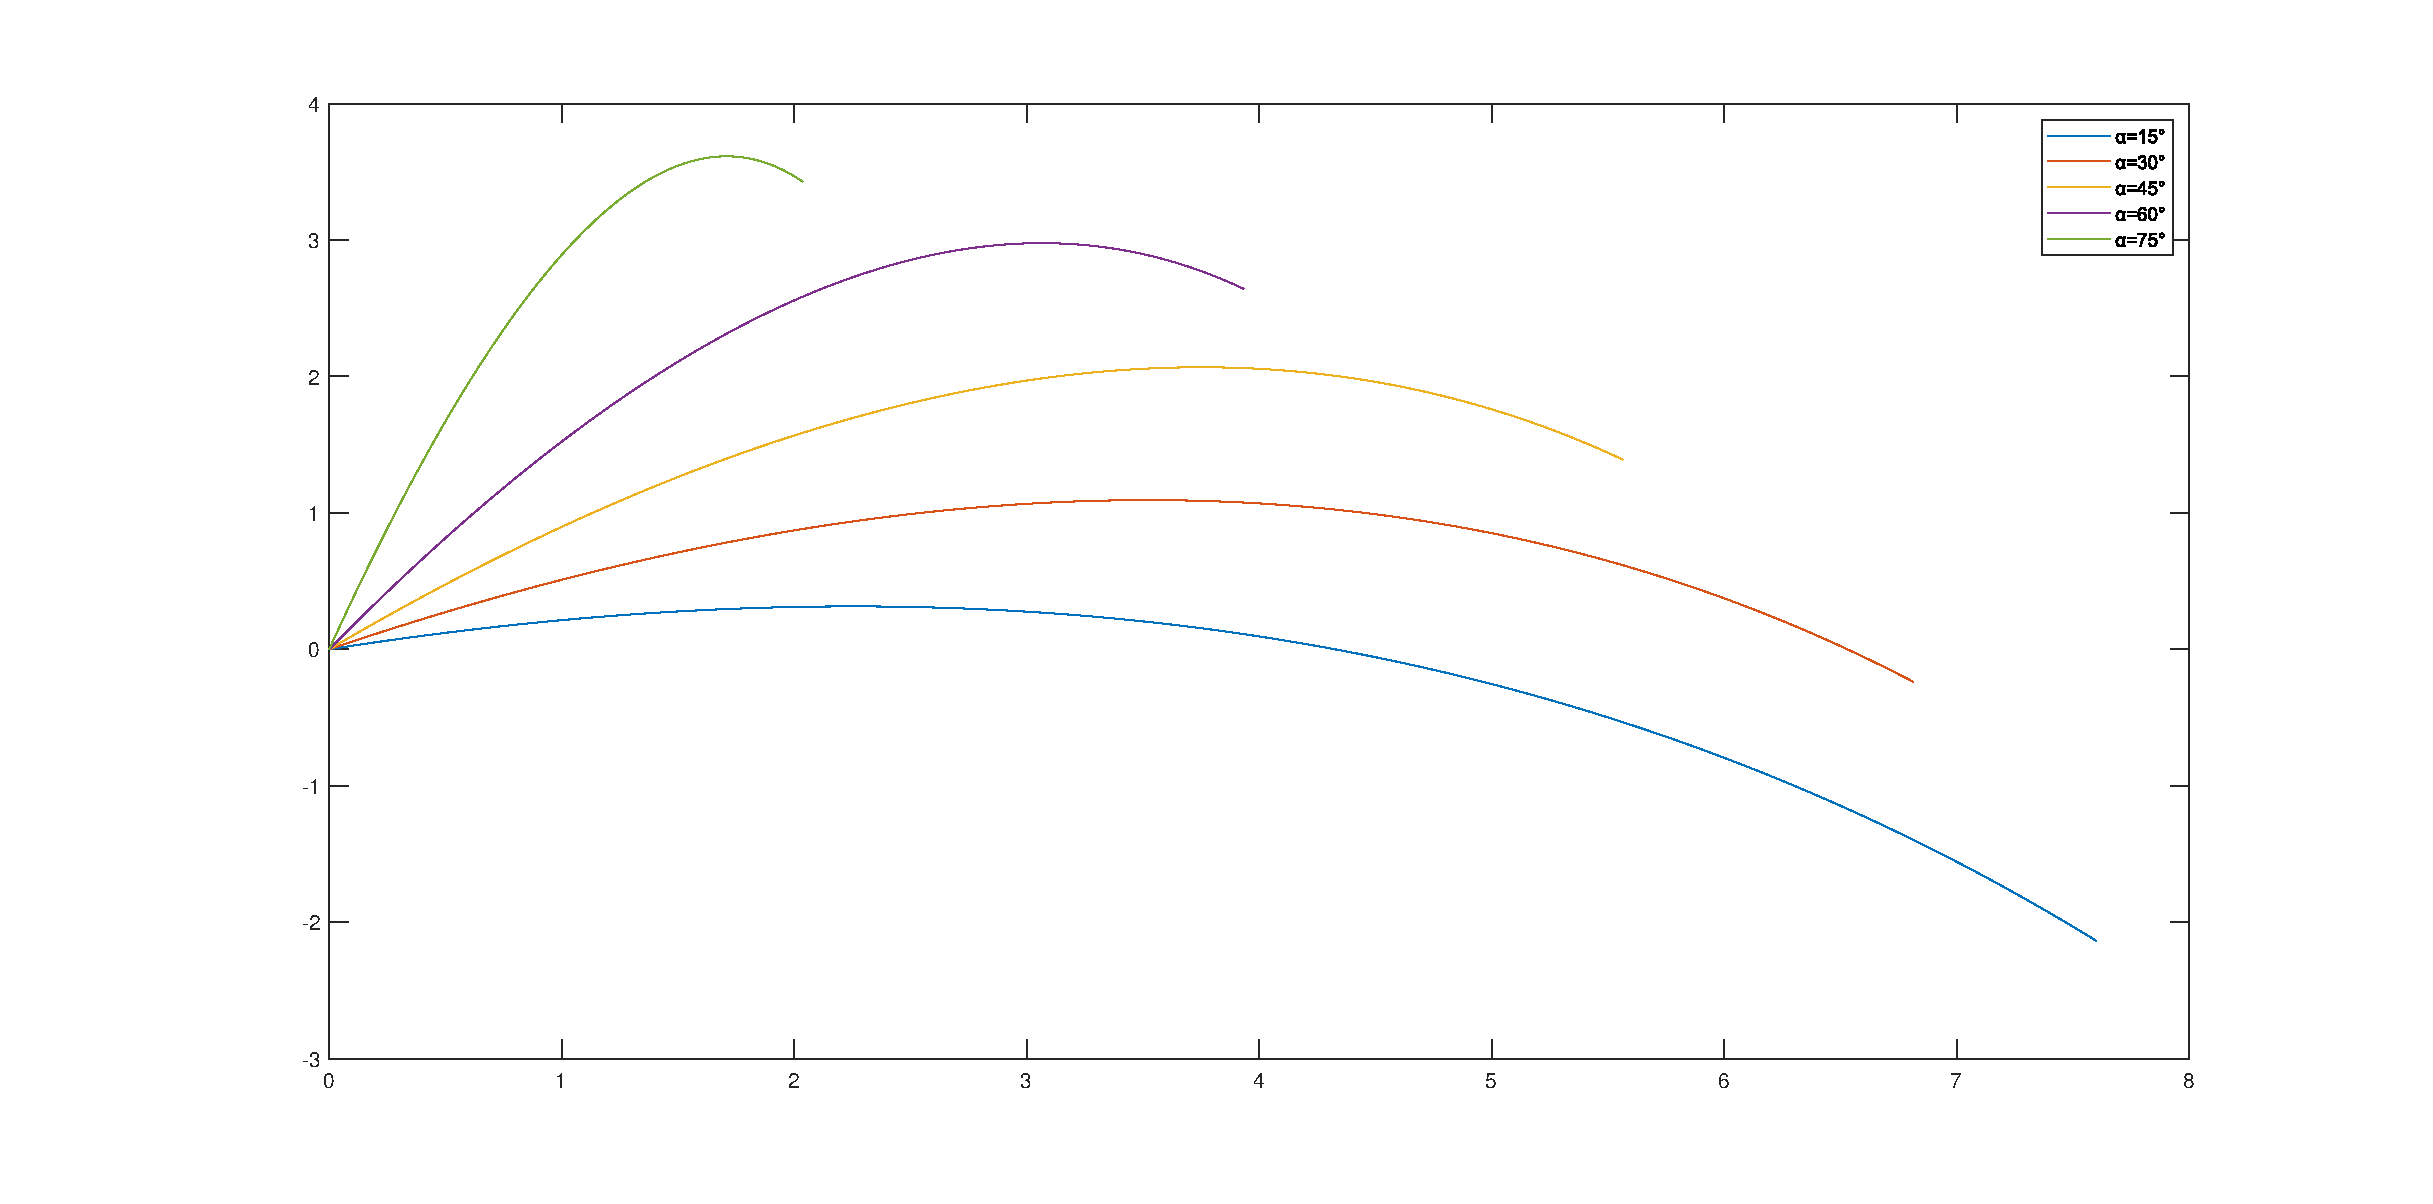
\includegraphics[width=1\linewidth]{2-1-3.eps}
    \caption{Trajectories for different $\alpha$ for linear drag}
\end{figure}

Qualitatively, the maximum height decreases as the angle decreases. For the same time period, the range of the trajectory decreases as the angle increases.

Besides, we can find the time dependence of the speed of the particle normed by $v=\sqrt{v_x^2+v_y^2}$.
\begin{figure}[H]
    \centering
    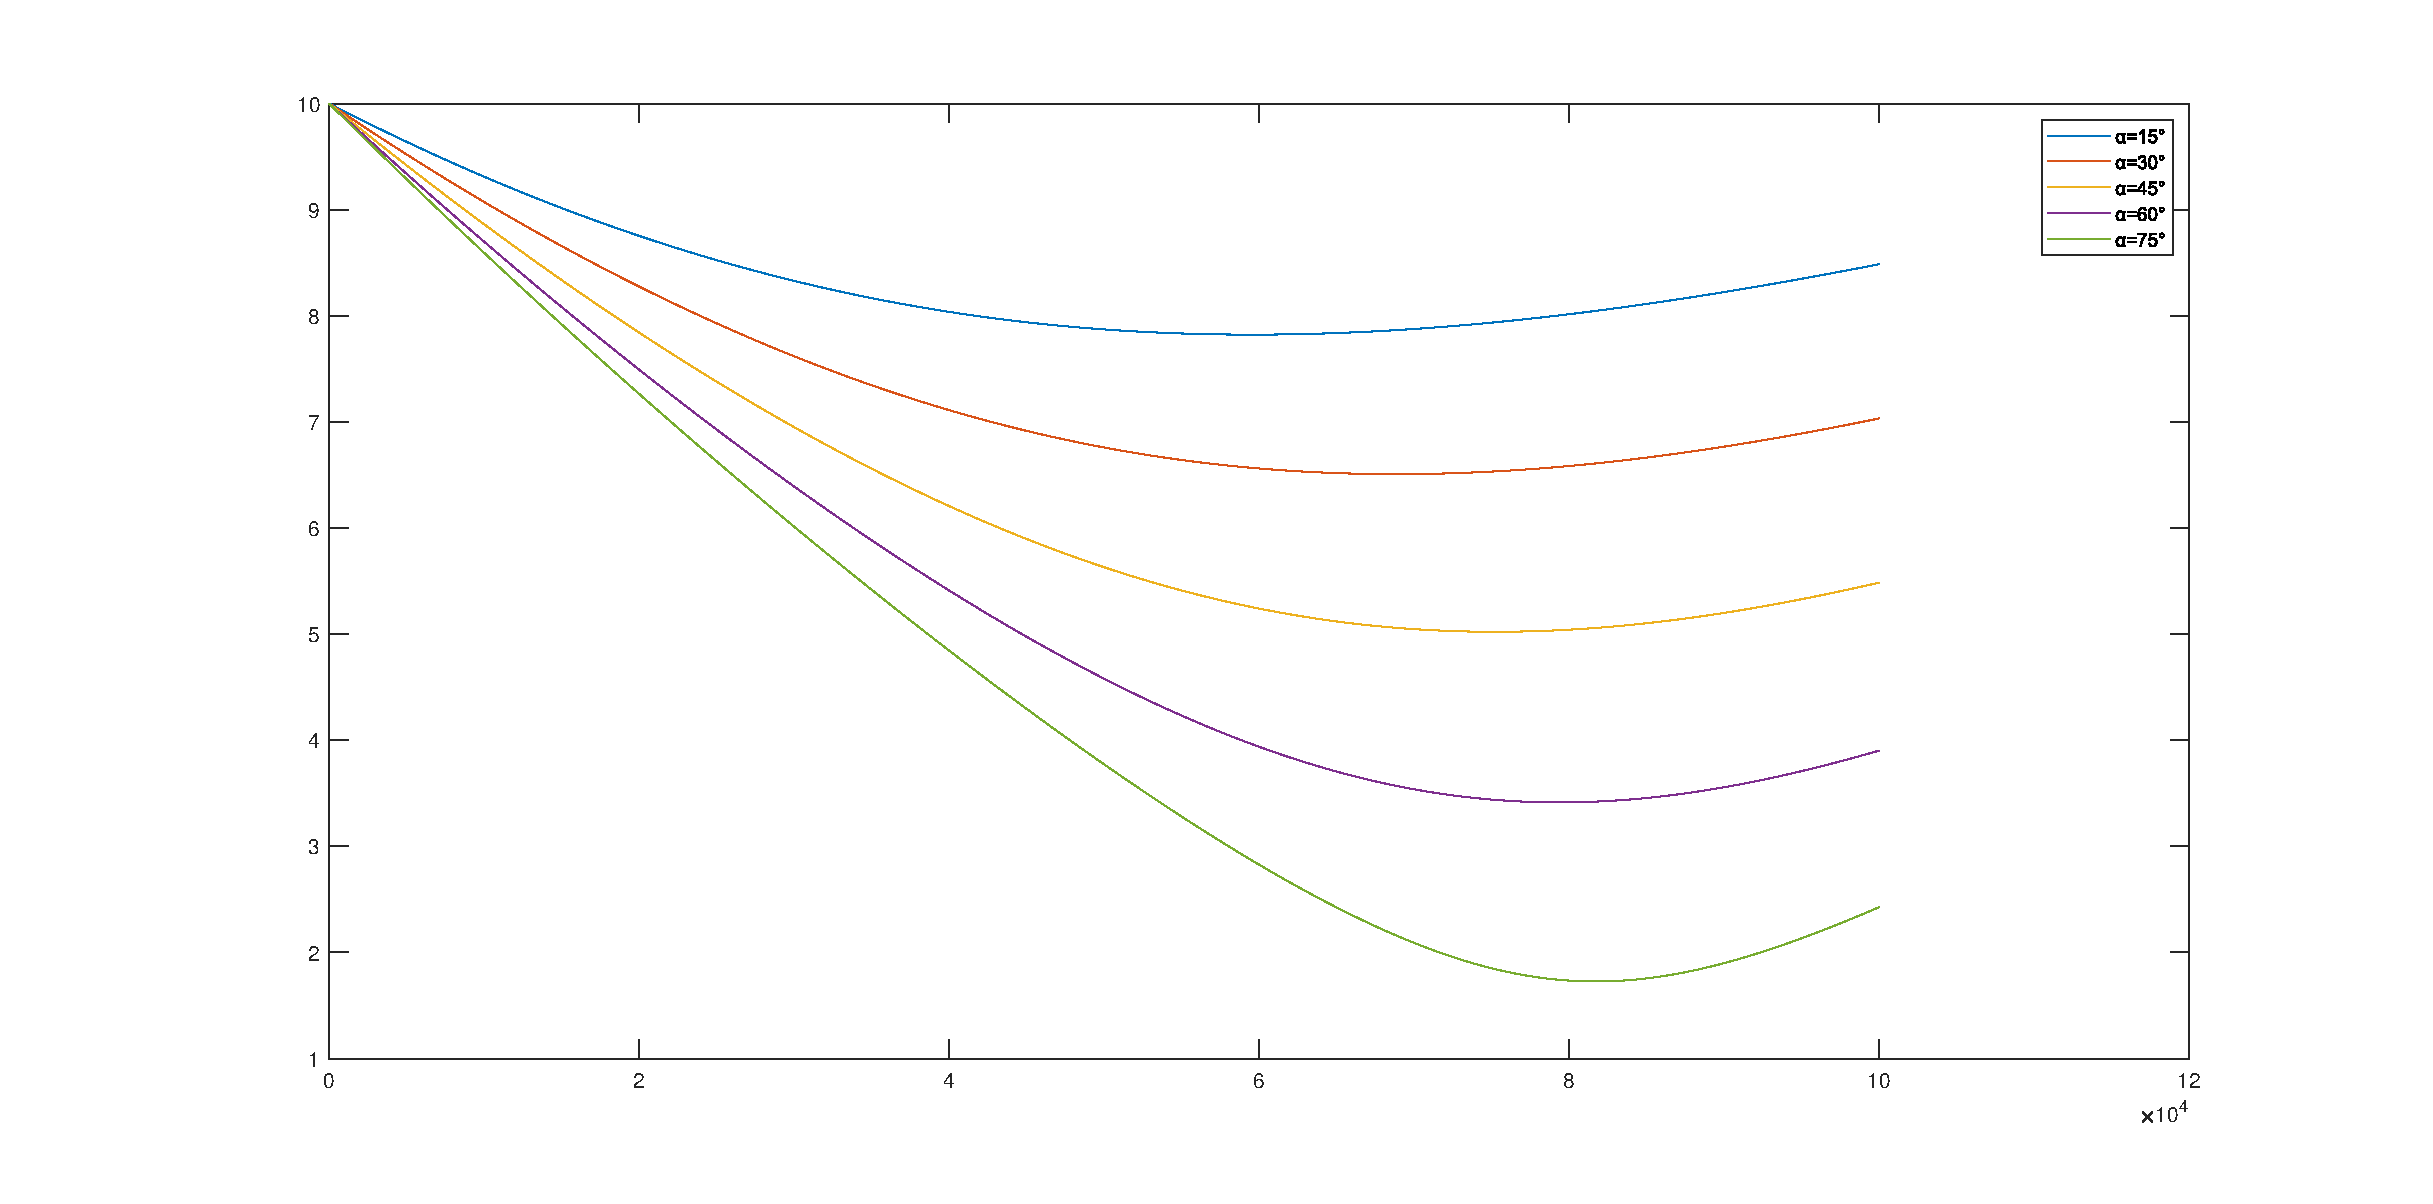
\includegraphics[width=1\linewidth]{2-1-4.eps}
    \caption{Time dependence of the speed for different $\alpha$ for linear drag}
\end{figure}

Reviewing the relationship from the figure above, we can find that as $\alpha$ increases, the minimum speed decreases, and the time when the speed approaches the minimum procrastinates. After the turning point, the vertical velocity increases from zero although the horizontal velocity continuously decreases due to linear air drag.

Similar to what we have done for taking different values of the angle $\alpha$, we examine the effect of the drag coefficient $\kappa$.
\begin{figure}[H]
    \centering
    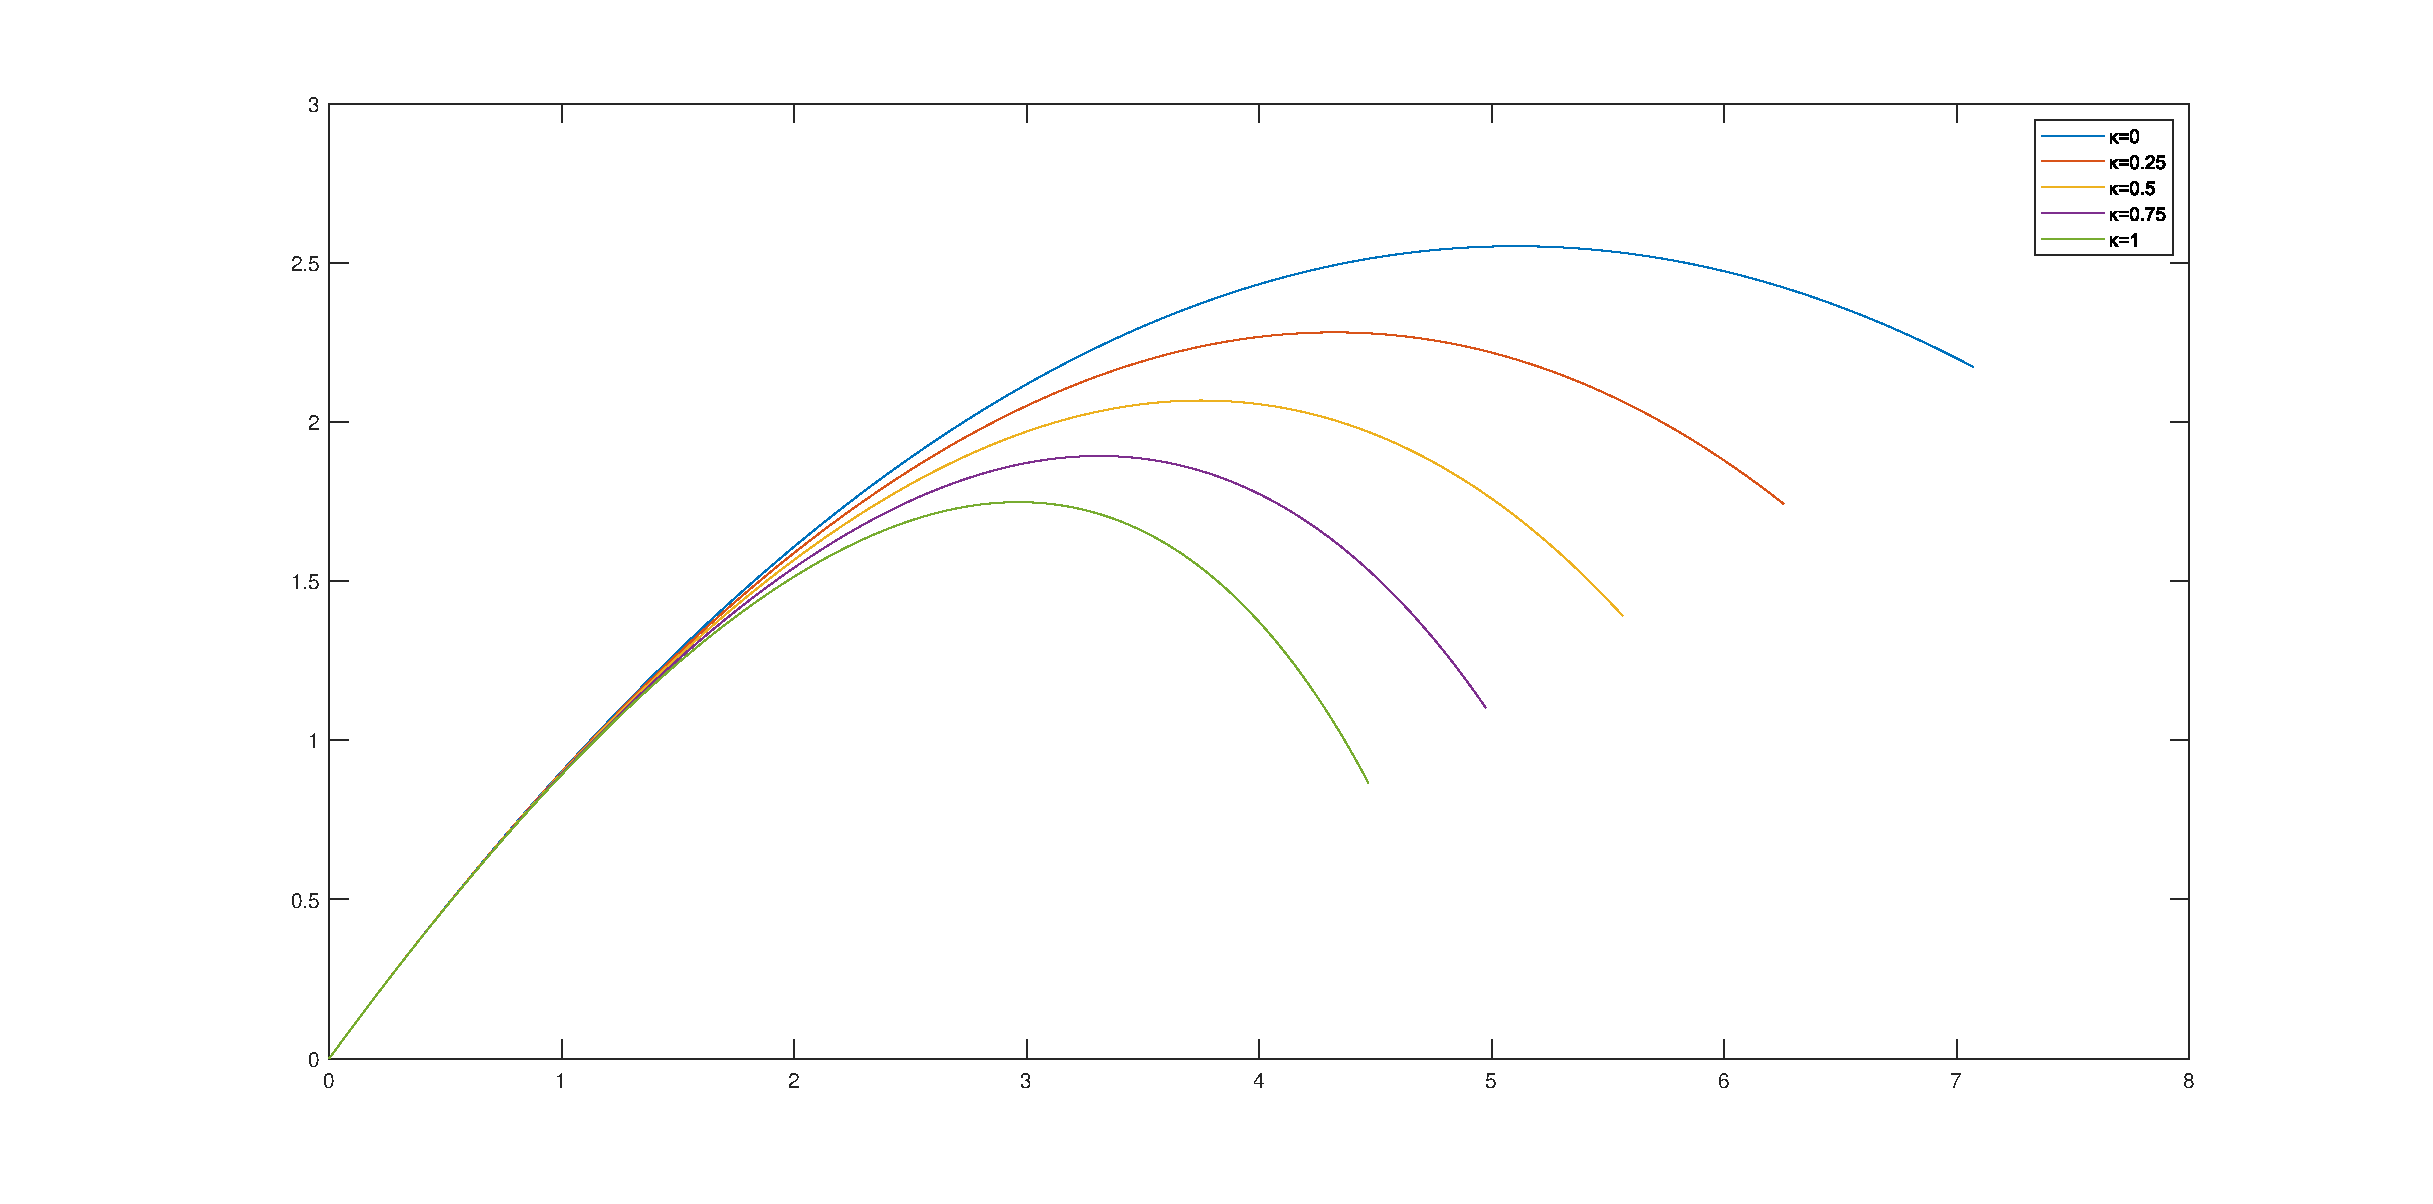
\includegraphics[width=1\linewidth]{2-1-5.eps}
    \caption{Trajectories for different $\kappa$ for linear drag}
\end{figure}

As the drag coefficient $\kappa$ increases, the range of the trajectory is less and so is the maximum height, because the air drag decreases the velocity of the particle for both $x$ and $y$ components.
\begin{figure}[H]
    \centering
    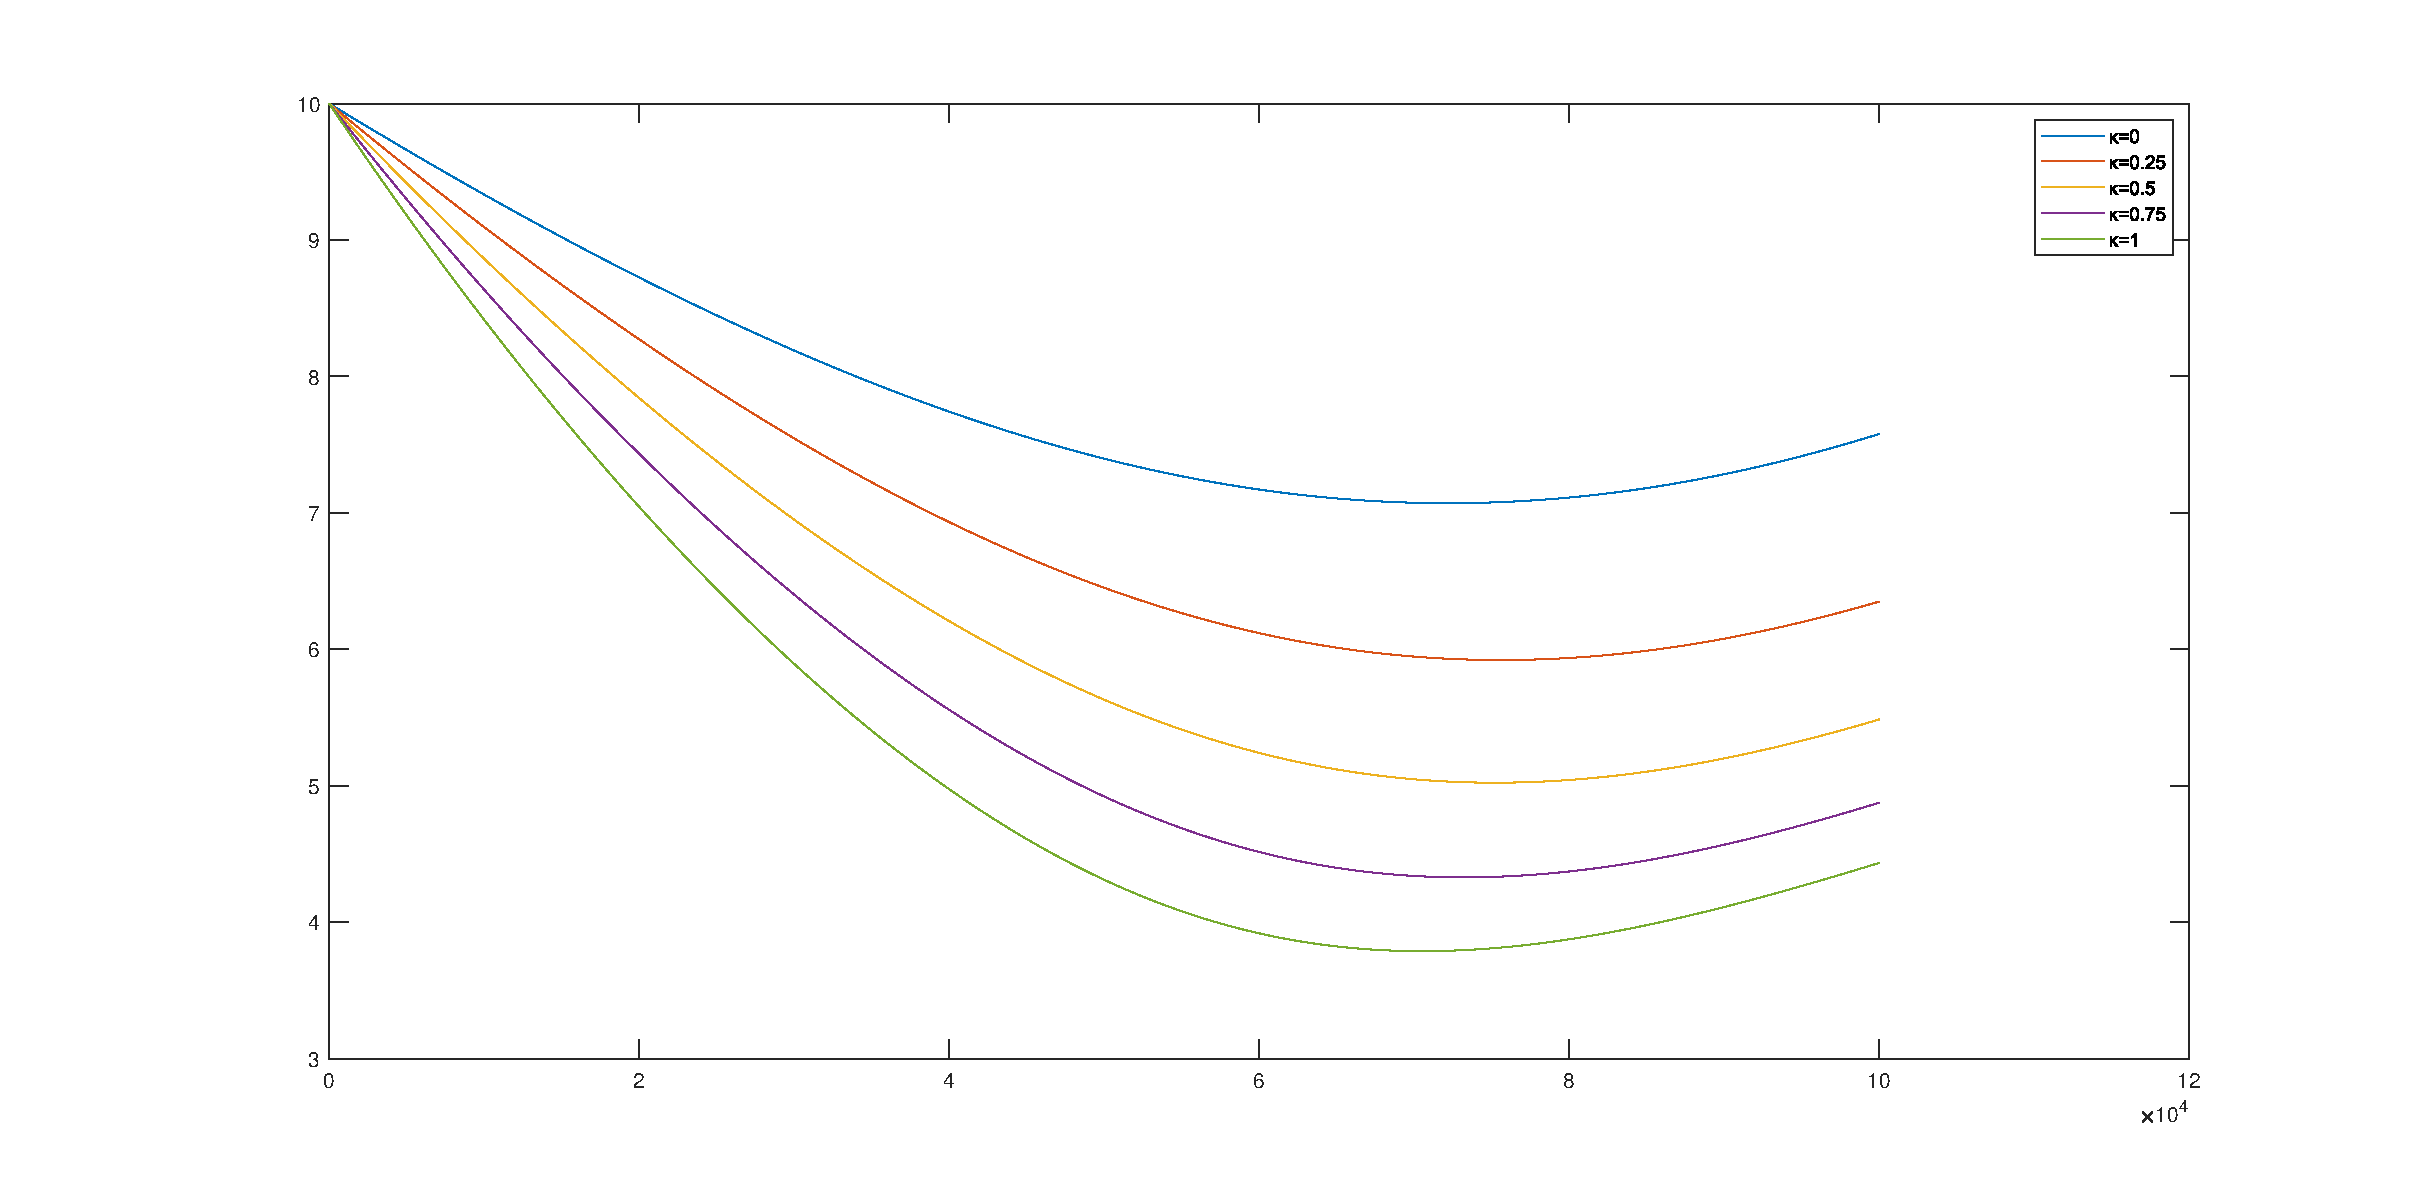
\includegraphics[width=1\linewidth]{2-1-6.eps}
    \caption{Time dependence of the speed for different $\kappa$ for linear drag}
\end{figure}

As the drag coefficient $\kappa$ increases, the minimum speed decreases and the time when the speed is minimized is less. Besides, there are no intersections among these curves.
\subsection{Quadratic Drag}
The acceleration of particles with quadratic drag are in proportion to the square of the velocity. Using Euler's method,
\begin{equation}
    F_x=m\Ddot{x}=-m\beta v_x^{*2}
\end{equation}

For velocity in the direction of $x$,
\begin{equation}
    v_{x,i+1}^*=v_{x,i}^*-\beta\left|v_i^*\right| v_{x,i}^*\Delta t=v_{x,i}^*-\beta\sqrt{v_{x,i}^{*2}+v_{y,i}^{*2}} v_{x,i}^*\Delta t
\end{equation}
then the velocity in the orthogonal base,
\begin{equation}
    v_{y,i+1}^*=v_{y,i}^*-(g+\beta\sqrt{v_{x,i}^{*2}+v_{y,i}^{*2}} v_{y,i}^*\Delta t
\end{equation}

For positions, they are the same as those for linear drag.
\begin{equation}
    x_{i+1}^*=x_i^*+v_{x,i}^*\Delta t
\end{equation}
and
\begin{equation}
    y_{i+1}^*=y_i^*+v_{y,i}^*\Delta t
\end{equation}
Hence, we have the recursive equations for velocity and position of the projectile for further numerical simulation.

To examine the sensitivity of the numerical result to the choice of $\Delta t$, we still choose three different values of $\Delta t$ 0.001 s, 0.0001 s, and 0.00001 s.
\begin{figure}[H]
    \centering
    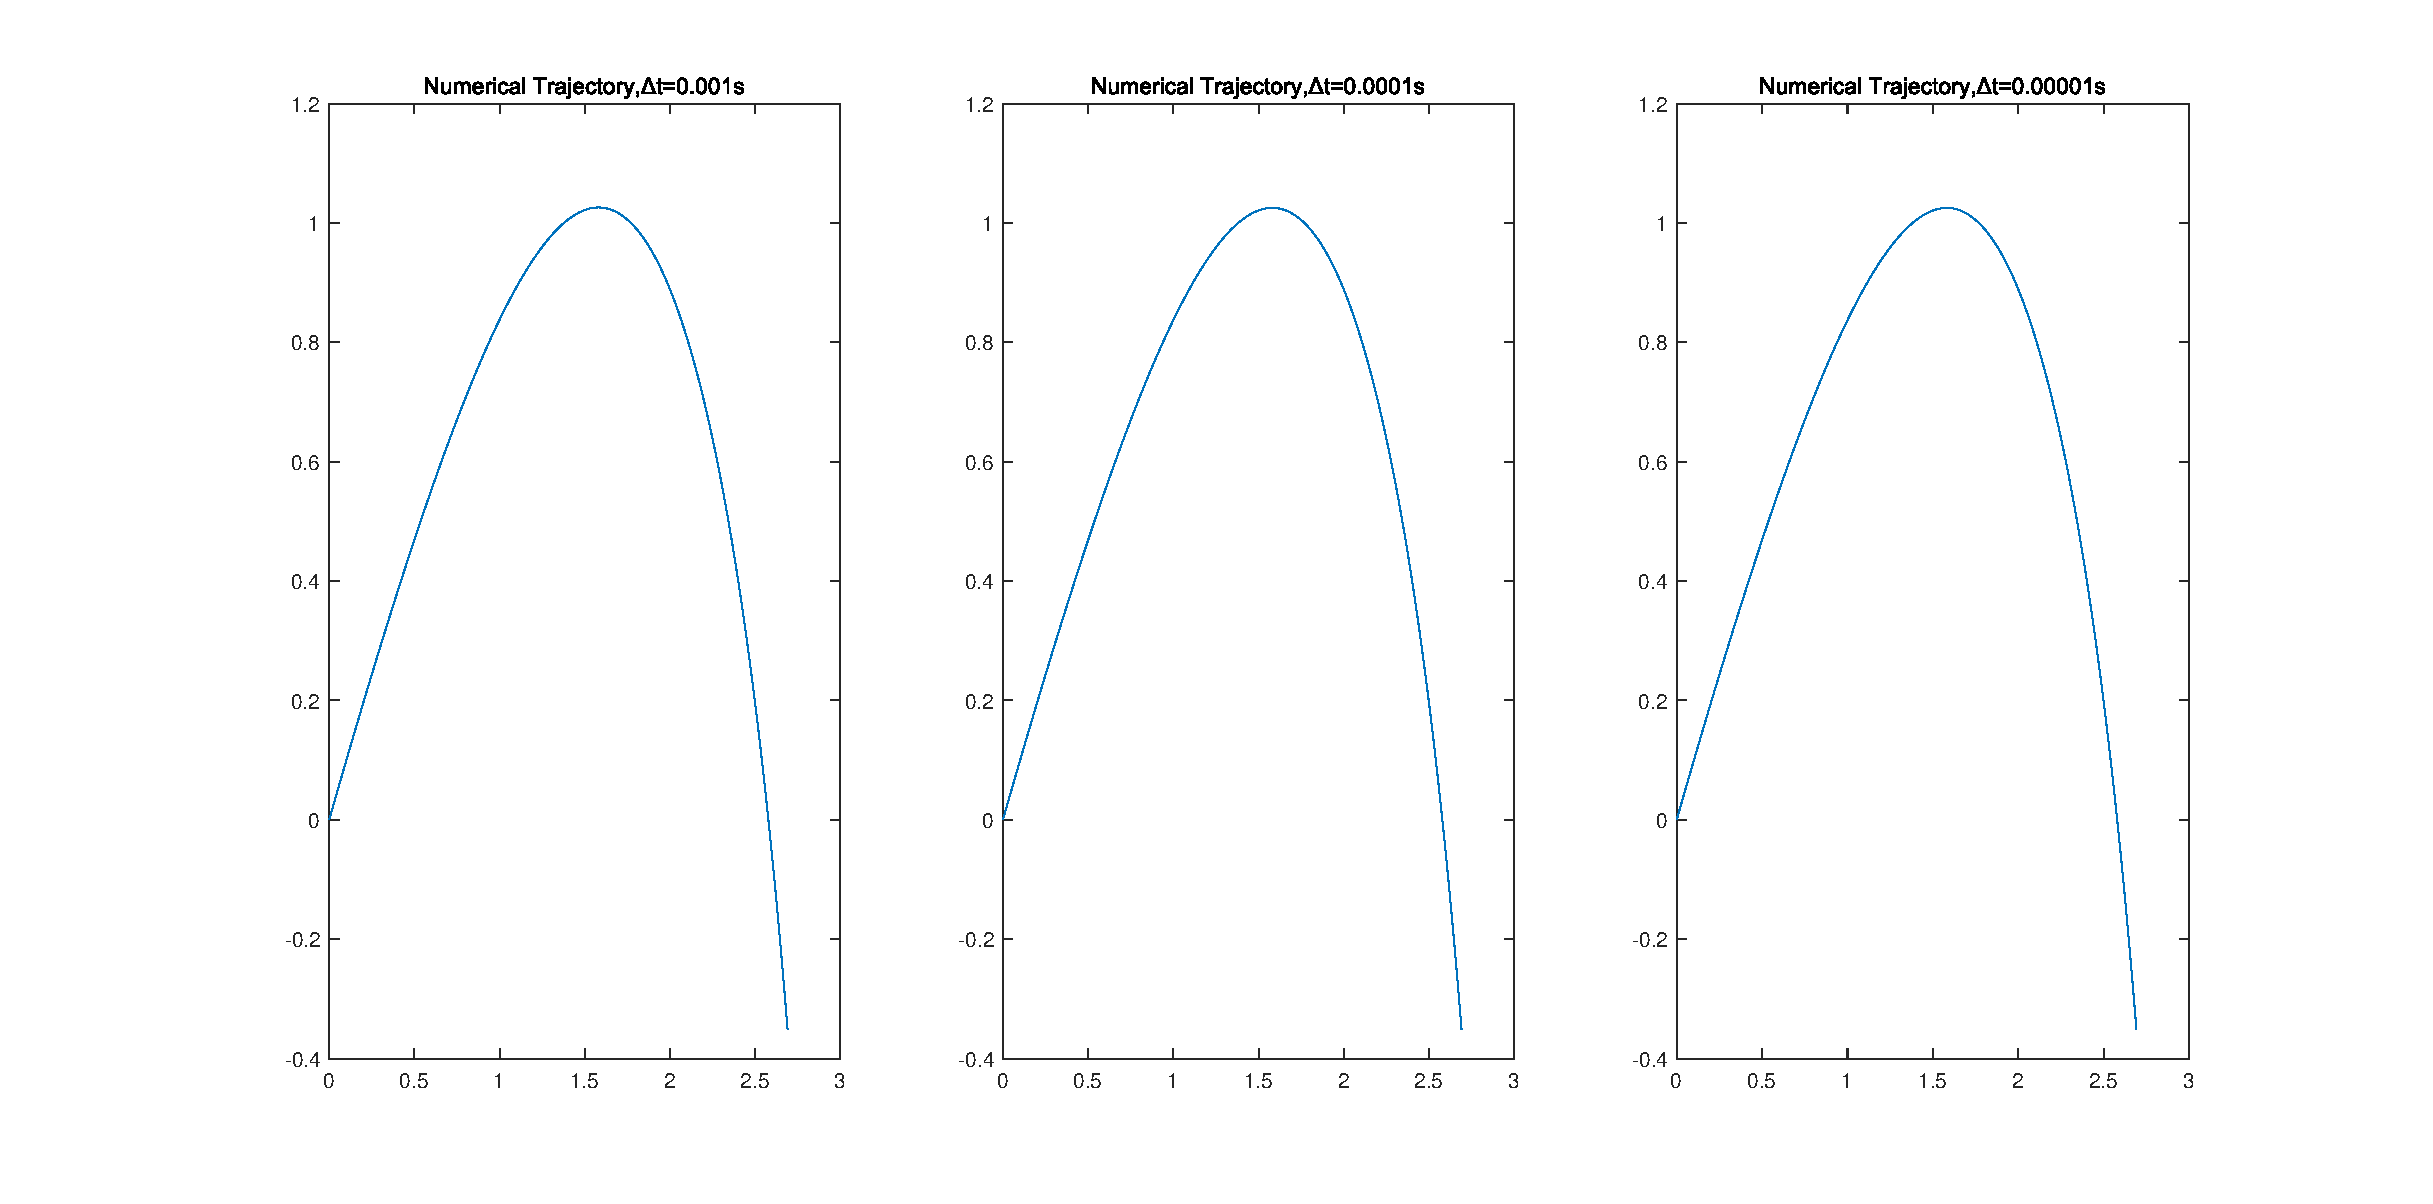
\includegraphics[width=1\linewidth]{2-2-1.eps}
    \caption{Trajectories for different $\Delta t$ for quadratic drag}
\end{figure}
Assuming the initial velocity $v_0=10$ m/s, $\alpha=45^\circ$, and $\beta=0.5$, we can plot the three trajectories for different values of $\Delta t$ and find that the numerical result is not quite sensitive to the choice of $\Delta t$ in this interval. If the choice of $\Delta t$ is too great, then the numerical result may vary obviously from the real situation.

Since it turns out that still the smaller the interval $\Delta t$ is, the better simulation for the solution we have. For different choices of the angle $\alpha$, we can plot the trajectories and find the differences.
\begin{figure}[H]
    \centering
    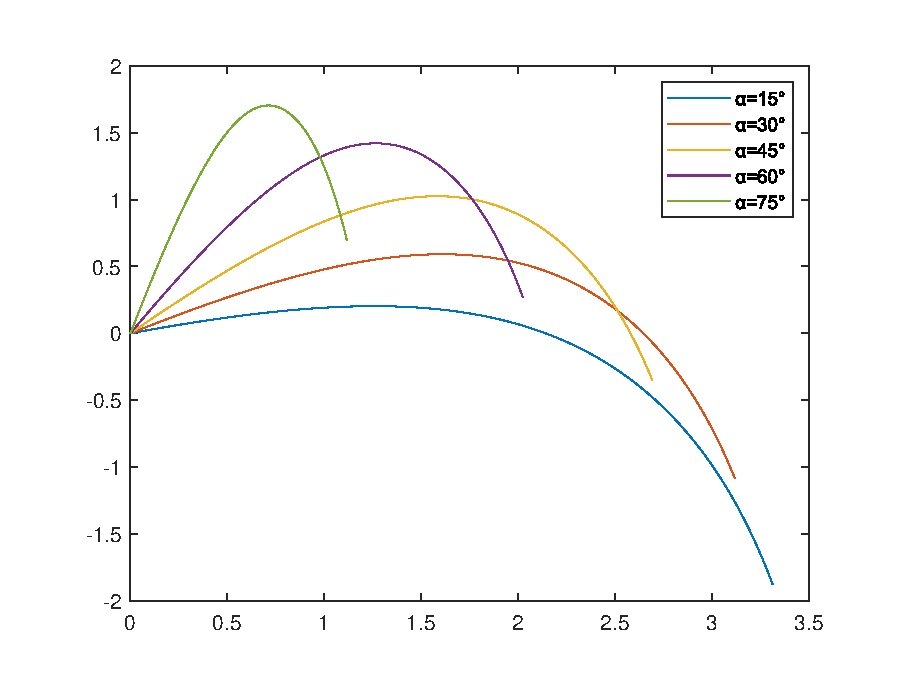
\includegraphics[width=1\linewidth]{2-2-2.eps}
    \caption{Trajectories for different $\alpha$ for quadratic drag}
\end{figure}
As the angle $\alpha$ increases, the range of the trajectory decreases and the maximum height increases comparing the 5 curves according to Figure 8.
\begin{figure}[H]
    \centering
    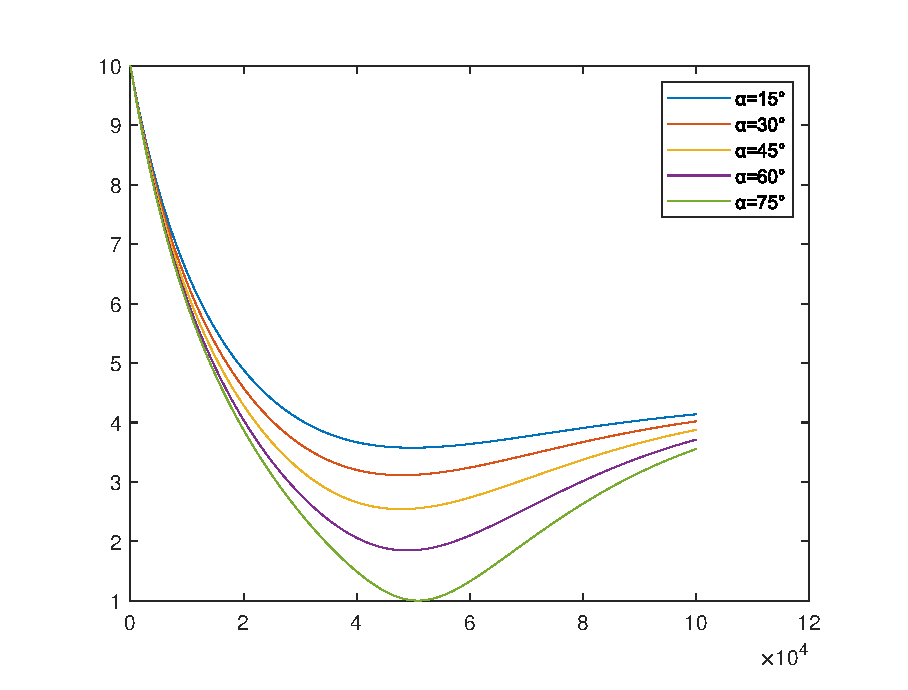
\includegraphics[width=1\linewidth]{2-2-3.eps}
    \caption{Time dependence of the speed for different $\alpha$ for quadratic drag}
\end{figure}
In Figure 9, as time $\alpha$ increases, the minimum speed decreases and the corresponding time increases. As time goes by, the speed decreases first and then increases.

On the other hand, fixing $alpha=45^\circ$ and choosing different values of drag coefficient $\kappa$ of a set \{0, 0.25, 0.5, 0.75, 1\}, we plot the trajectories and corresponding time dependencies.
\begin{figure}[H]
    \centering
    \includegraphics[width=1\linewidth]{2-2-4.eps}
    \caption{Trajectories for different $\kappa$ for quadratic drag}
\end{figure}
As the angle $\kappa$ increases, the range of the trajectory decreases and the maximum height also decreases comparing the 5 curves according to Figure 10.
\begin{figure}[H]
    \centering
    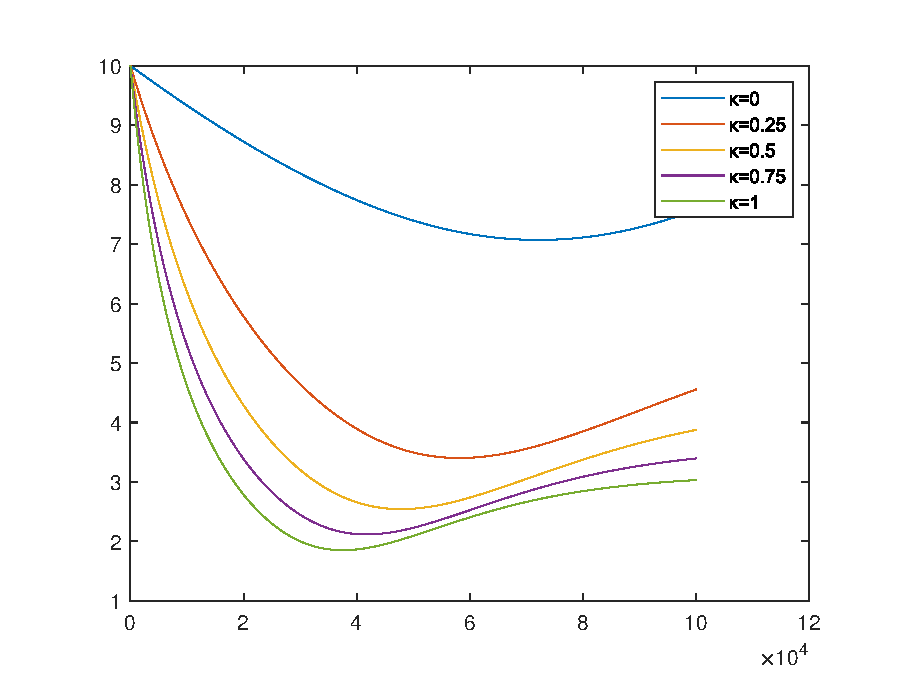
\includegraphics[width=1\linewidth]{2-2-5.eps}
    \caption{Time dependence of the speed for different $\kappa$ for quadratic drag}
\end{figure}
As  time $\kappa$ increases, the minimum speed decreases while the corresponding time $t$ increases. The differences between speed when $\kappa=0$ and $\kappa=0.25$ is quite great that the quadratic drag plays a more important role for smaller value of drag coefficient.
\subsection{Comparison between no drag, linear drag, and quadratic drag}
Choosing the set of initial conditions that $\alpha=45^\circ$, $\beta=\kappa=0.5$, and $v_0=10$ m/s, we would like to plot the three situations no drag, linear drag, and quadratic drag in the same graph.

For linear drag, calculating by Eq.22 and Eq.23, $v_x=4.2888$ m/s and $v_y=-3.4203$ m/s. The terminal speed is $v=5.4857$ m/s. By the relationship when balancing
\begin{equation}
    \kappa v=\beta v^2
\end{equation}
When $\kappa=0.5$, $\beta=0.09114657$. We can thence plot the trajectories in Figure 12, both drags with the same terminal speed.
\begin{figure}[H]
    \centering
    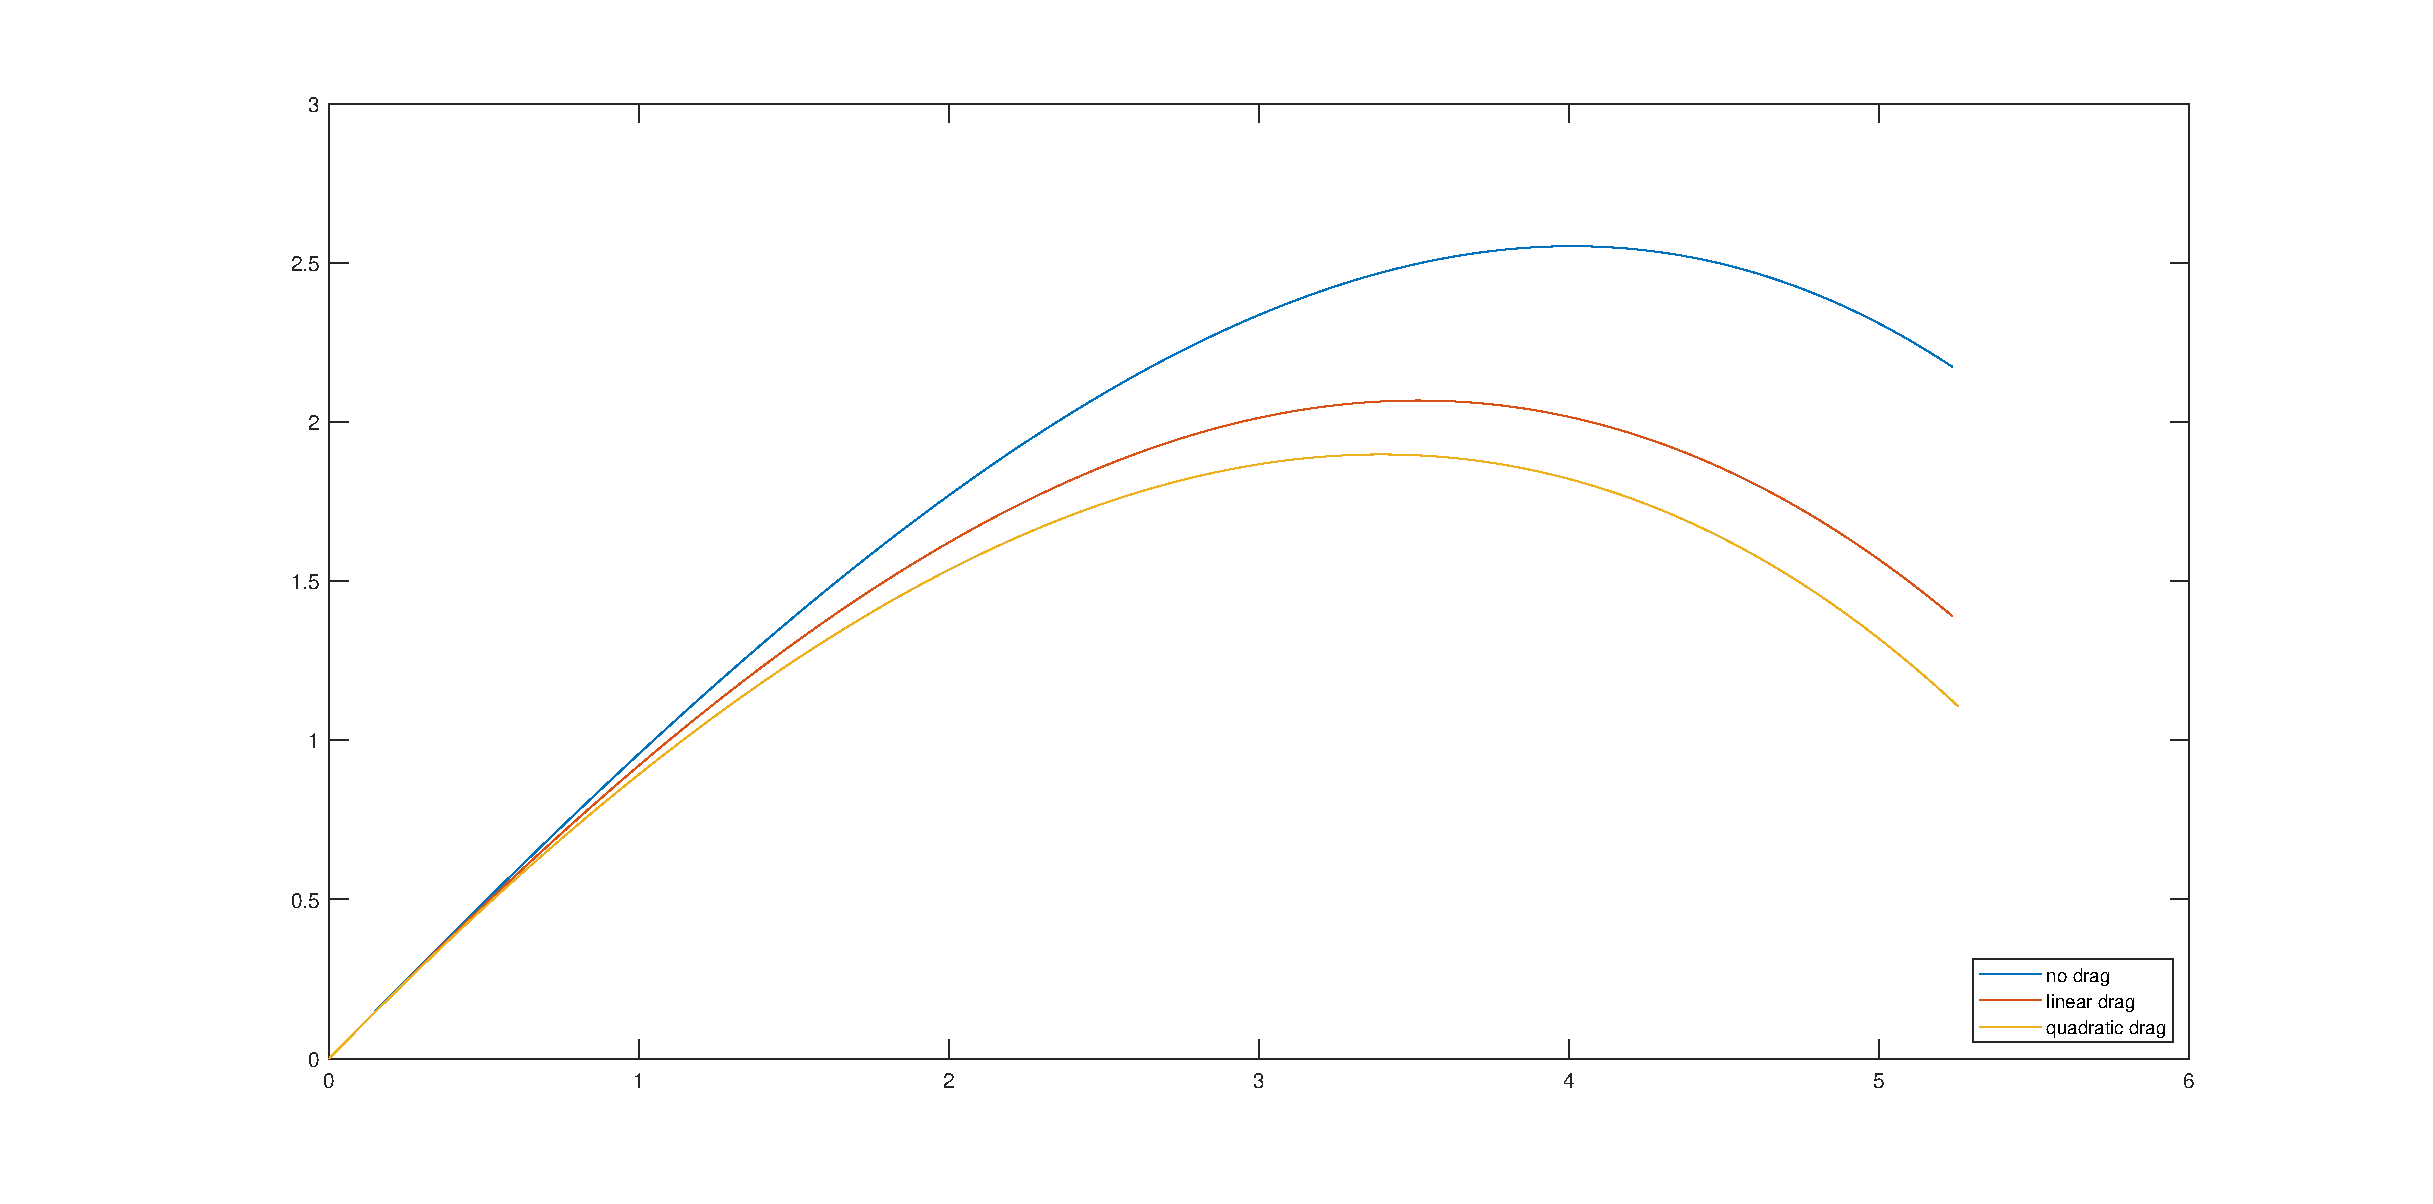
\includegraphics[width=1\linewidth]{2-3.eps}
    \caption{Trajectories with the same terminal drag speed for no drag, linear drag, and quadratic drag}
\end{figure}
From Figure 12, we can find that both drags decreases the y coordinates with the same x coordinates relatively during the motion. Furthermore, the quadratic drag gives a higher drag effects on the motion of the particle than linear drag.
\subsection{Heun's Method}
In this part, we will apply Heun's Method to discuss the projectile motion with air drag. These are our additional part of this research. We have to consider $k_1$ and $k_2$ with respect to each i. 
\begin{equation}
    k_{1}(x_{x,i-1})=v_{x,i-1}^*
\end{equation}
\begin{equation}
    k_{2}(x_{x,i-1})=v_{x,i-1}^* + a_{x,i-1}\Delta t
\end{equation}
Then we could estimate $x_{x,i-1}$ as follows:
\begin{equation}
    x_{x,i}^*=x_{x,i-1}^*+\frac{1}{2}(k_{1}+k_{2})\Delta t=x_{x,i-1}^*+\frac{1}{2}(v_{x,i-1}^*+v_{x,i-1}^* + a_{x,i-1}^*\Delta t)\Delta t
\end{equation}
\begin{equation}
   x_{x,i}^* =x_{x,i-1}^*+\frac{1}{2}(v_{x,i-1}^*+v_{x,i-1}^*-\kappa v_{x,i-1}^*\Delta t)\Delta t
\end{equation}
Then we could discuss the estimate of $v_{x,i-1}$ as follows:
\begin{equation}
    k_{1}(v_{x,i-1})=-\kappa v_{x,i-1}^*
\end{equation}
\begin{equation}
    k_{2}(v_{x,i-1})=-\kappa v_{x,i-1}^* + \kappa^2 v_{x,i-1}^*\Delta t
\end{equation}
\begin{equation}
    v_{x,i}^*=v_{x,i-1}^*+\frac{1}{2}(k_{1}+k_{2})\Delta t
   =v_{x,i-1}^*+\frac{1}{2}(-\kappa v_{x,i-1}^*-\kappa v_{x,i-1}^* + \kappa^2v_{x,i-1}^*\Delta t)\Delta t
\end{equation}
Then we consider the y-direction as follows:  
\begin{equation}
    k_{1}(x_{y,i-1})=v_{y,i-1}^*
\end{equation}
\begin{equation}
    k_{2}(x_{y,i-1})=v_{y,i-1}^* +(-g-\kappa v_{y})\Delta t
\end{equation}
\begin{equation}
    x_{y,i}^*=x_{y,i-1}^*+\frac{1}{2}(k_{1}+k_{2})\Delta t
   =x_{y,i-1}^*+\frac{1}{2}(v_{y,i-1}^*+v_{y,i-1}^* +(-g-\kappa v_{y})\Delta t)\Delta t
\end{equation}
\clearpage
\begin{equation}
    k_{1}(v_{y,i-1})=-g-\kappa v_{y,i-1}^*
\end{equation}
\begin{equation}
    k_{2}(v_{y,i-1})=-g-\kappa v_{y,i-1}^* +(\kappa g+\kappa^2 v_{y,i-1})\Delta t 
\end{equation}
\begin{equation}
    v_{y,i}^*=v_{y,i-1}^*+\frac{1}{2}(k_{1}+k_{2})\Delta t
   =v_{y,i-1}^*+\frac{1}{2}(-g-\kappa v_{y,i-1}^*+-g-\kappa v_{y,i-1}^* +(\kappa g+\kappa^2 v_{y,i-1})\Delta t )\Delta t
\end{equation}
Then we get the recursive equations for x and v for both x and y directions. Following figures are the trajectory and the t vs. v graph. We take five sets of $\kappa$ to do the plot.\newline
\begin{figure}[h]
    \centering
    \includegraphics[width=1\linewidth]{position121.png}
    \caption{trajectory 1 and 2}
    \label{fig:my_label}
\end{figure}
\begin{figure}
    \centering
    \includegraphics[width=1\linewidth]{position34.png}
    \caption{trajectory 3 and 4}
    \label{fig:my_label}
\end{figure}
\begin{figure}
    \centering
    \includegraphics[width=1\linewidth]{postion5.png}
    \caption{trajectory 5}
    \label{fig:my_label}
\end{figure}
\begin{figure}
    \centering
    \includegraphics[width=1\linewidth]{velocity12.png}
    \caption{velocity 1 and 2}
    \label{fig:my_label}
\end{figure} 
\begin{figure}[htbp]\centering\includegraphics[height=9cm,width=16cm]{velocity34.png}
\caption{velocity 3 and 4}
\end{figure}   
\begin{figure}[htbp]\centering\includegraphics[height=9cm,width=10cm]{velocity5.png}
\caption{velocity 5}
\end{figure}
\clearpage
\section{Simple harmonic oscillator}
In this part, we will use two different methods, Euler's and Heun's methods to solve the problem of simple harmonic motion. We set the initial conditions as $x(0)=0.5 m$, $v_{x}(0)=1m/s$. Suppose the angular frequency $\omega_{0}$ satisfies that $\omega_{0}=1.5 s^{-1}$. Furthermore, we assume the mass of the oscillator is 1 kg so that we can easily calculated the mechanical energy of the oscillation system.
\subsection{Euler's Method}
Applying Euler's equation of motion, we can obtain equation
\begin{equation}
	x_{i}^*=x_{i-1}^*+v_{x,i-1}^*\Delta, 
\end{equation}
and
\begin{equation}
	v_{i}^*=v_{i-1}^*+a_{x,i-1}^*\Delta t.
\end{equation}
The notation `*' means that the value is an approximated one. Besides, we know that in the simple harmonic motion, we have
\begin{equation}
    \Ddot{x}=-\omega_{0}^2x,
\end{equation}
where the secondary derivative of the position is actually the acceleration of the oscillator. Thus, we can obtain from Eq.46 that
\begin{equation}
    v_{x,i}^*=v_{x,i-1}^*-\omega_{0}^2x_{i-1}\Delta t.
\end{equation}
This equation together with Eq.(2) can form two recursive equations for velocity and the position of the oscillator when the initial values are given. Utilizing the recursive equations, we can plot the trajectory of the oscillator through MATLAB.
We set the value of $\Delta t$ as 0.01, and then plot 1000 points (green points) of $x$ from $t=0$ to $t=10$ to show the trajectory (shown in Figure 1). The trajectory is plotted in both configuration and phase space. In the configuration space, the x-axis refers to time and the y-axis refers to the position. In the phase space, the x-axis refers to position and the y-axis refers to velocity.\\~\\
Furthermore, we want to analyze the impact of the value of $\Delta t$ on the trajectory plotted using Euler's Method. So on the same graph, we choose $\Delta t=0.02$ to plot 500 points (yellow points) and $\Delta t=0.05$ to plot 200 points (blue points) so that the final time is the same. The three trajectories are shown in Figure 2.\\
\begin{figure}[htbp]
\centering
\subfigure[configuration space]{
\includegraphics[height=7cm,width=7cm]{3-1-1.png}
}
\subfigure[phase space]{
\includegraphics[height=7cm,width=7cm]{3-1-3.png}
}
\caption{Trajectory plotted using Euler's Method}
\end{figure}
\begin{figure}[htbp]
\centering
\subfigure[configuration space]{
\includegraphics[height=7cm,width=7cm]{3-1-2.png}
}
\subfigure[phase space]{
\includegraphics[height=7cm,width=7cm]{3-1-4.png}
}
\caption{Different trajectory]ies for different $\Delta t$}
\end{figure}
\newpage
Obviously, the numerical result is sensitive to the choice of the step $\Delta t$.  The analytical formulas of the position and velocity of a oscillator are sine and cosine functions, represented in the following way
\begin{align}
x=A\sin(\omega t+\phi) && v=\omega A\cos(\omega t+\phi).
\end{align}
This also indicates that the trajectory in the phase space should be a ellipse. Comparing the result in Figure 2 with the analytical formulas, we can find out that the larger the step $\Delta t$ is, the more divergent the trajectory from the theoretical value. Hence we can deduce that the smaller the step we choose, the more accurate the result we are going to obtain.\\~\\
Furthermore, we are interested in the mechanical energy of the oscillation system. The energy for every moment is calculated by the formula
\begin{equation}
    E(t)=\frac{1}{2}m\omega_{0}^2x^2+\frac{1}{2}mv^2.
\end{equation}
We choose $\Delta t=0.01$ and use the previous method to figure out the velocity and position at each step. The we calculate the mechanical energy at every step and plot 1000 points to make a graph (shown in Figure 3). The x-axis refers to the time and the y-axis refers to the energy.
\begin{figure}[htbp]
\centering
\includegraphics[width=0.8\linewidth]{3-1-5.png}
\caption{The graph of the mechanical energy}
\end{figure}\\
From the graph we can see that the mechanical energy of the oscillator is increasing slowly. However, we can have conjecture that the mechanical energy f the system is conversed. This is because the graph is plotted using Euler's Method, which is an approximation to the real situation. And from the previous conclusion we can know that the velocity and position is much larger than the theoretical value if the step $\Delta t$ is too large, so it's reasonable to make such a conjecture. Then we need to prove it analytically.\\~\\
From Eq.2 and Eq.5, we can obtain that for any i$\ge$1, we can represent the energy function 
\begin{equation}
    E(t_{i})=\frac{1}{2}m\omega_{0}^2(x_{i-1}^*+v_{x,i-1}^*\Delta t)^2+\frac{1}{2}m(v_{x,i-1}^*-\omega_{0}^2x_{i-1}\Delta t)^2.
\end{equation}
By uniting similar terms, we can obtain that
\begin{equation}
    E(t_{i})=\frac{1}{2}m\omega_{0}^2((x_{i-1}^*)^2\omega_{0}^2+v_{x,i-1}^2)(1+\omega_{0}^2\Delta t^2).
\end{equation}
Since 
\begin{equation}
    E(t_{i-1})=\frac{1}{2}m\omega_{0}^2((x_{i-1}^*)^2\omega_{0}^2+v_{x,i-1}^2),
\end{equation}
We can get a recursion formula for $E(t_i)$
\begin{equation}
    E(t_{i})=(1+\omega_{0}^2\Delta t^2)E(t_{i-1}).
\end{equation}
Thus, we can write that 
\newline\centerline{$E(t_{0})=\frac{1}{2}m\omega_{0}^2((x_{0}^*)^2\omega_{0}^2+v_{x,0}^2)$}
\newline\centerline{$E(t_{1})=\frac{1}{2}m\omega_{0}^2((x_{1}^*)^2\omega_{0}^2+v_{x,0}^2)(1+\omega_{0}^2\Delta t^2)$}
\newline\centerline{$E(t_{2})=\frac{1}{2}m\omega_{0}^2((x_{2}^*)^2\omega_{0}^2+v_{x,0}^2)(1+\omega_{0}^2\Delta t^2)^2$}
\newline\centerline{...}
\newline\centerline{$E(t_{n})=\frac{1}{2}m\omega_{0}^2((x_{n}^*)^2\omega_{0}^2+v_{x,0}^2)(1+\omega_{0}^2\Delta t^2)^n.$}\\~\\
For this result, we can find out that if our $\Delta t$ converges to 0, our energy will keep the same, which follows the regular energy pattern of simple harmonic motion. If the $\Delta t$ does not come close to 0, the energy will come to infinity with the increase of n. This coincide with our observation on the graph plotted using Euler's Method. Thus, Euler's approximation only works when $\Delta t$ is sufficiently small, and when the step $\Delta t$ converges to 0, we can get the theoretical value of the approximation.
\clearpage
\subsection{Heun's Method}
Applying Heun's method, for any i$\ge$1, we can calculate the slope $k_1$ of the left end and the slope $k_2$ of the right end of the interval for each step $\Delta t$
\begin{align}
	k_{1}(x_{i-1})=v_{x,i-1}^* && k_{2}(x_{i-1})=v_{x,i-1}^*-\omega_{0}^2x_{i-1}\Delta t.
\end{align}
Therefore, we can get the recursive equation for the position as
\begin{equation}
    x_{i}=x_{i-1}+\frac{1}{2}(k_{1}+k_{2})\Delta t=x_{i-1}+\frac{1}{2}(v_{x,i-1}^*+v_{x,i-1}^*-\omega_{0}^2x_{i-1}\Delta t)\Delta t.
\end{equation}
Similarly, we apply Heun's method to the velocity, then we have the following equations:
\begin{equation}
    k_{1}(v_{x,i-1})=-\omega_{0}^2x_{i-1},
\end{equation}
\begin{equation}
    k_{2}(v_{x,i-1})=-\omega_{0}^2(x_{i-1}+v_{x,i-1}\Delta t),
\end{equation}
\begin{equation}
    v_{x,i}=v_{x,i-1}+\frac{1}{2}(k_{1}+k_{2})\Delta t=v_{x,i-1}-\frac{1}{2}\omega_{0}^2\Delta t(x_{i-1}+x_{i-1}+v_{x,i-1}\Delta t).
\end{equation}
Utilizing the recursive equations Eq.56 and Eq.59, we are able to plot the trajectory of the oscillator. Since in section 3.1 we have concluded that the accuracy of the approximation done by Euler's Method decreases as the step $\Delta t$ increases, we would like to choose the largest step we have used in section 3.1, $\Delta t=0.05$, to plot 200 points of the trajectory using Heun's Method.\\~\\
We have known the the general equation for the motion of a harmonic oscillation is a sine or cosine function, which can be represented as
\begin{equation}
	x=A\sin(\omega t+\phi).
\end{equation}
Since the initial condition is given that $x(0)=0.5$ and $v(0)=1$, we can calculated the maximum amplitude through energy conservation:
\begin{equation}
	\frac{1}{2}mv_0^2+\frac{1}{2}m\omega_0^2 x_0^2=\frac{1}{2}m\omega_0^2 A^2.
\end{equation}
Hence the theoretical amplitude is $A=\frac{5}{6}m$. The initial phase $\phi$ is calculated by putting in initial terms, and the result is $\phi=\arcsin0.6$. The corresponding equation for velocity can be calculated by taking derivative of the position function.
\begin{equation}
	v=\omega A\cos(\omega t+\phi).
\end{equation}
Then we are able to plot the analytical result of the trajectory. This time, we would like to plot the trajectory approximated through Euler's Method and the trajectory approximated through Heun's Method on one figure, together with the trajectory calculated through analytical results (shown in Figure 4).
\newpage
\begin{figure}[htbp]
\centering
\subfigure[configuration space]{
\includegraphics[height=7cm,width=7cm]{3-2-1.png}
}
\subfigure[phase space]{
\includegraphics[height=7cm,width=7cm]{3-2-2.png}
}
\caption{Trajectories plotted using different methods}
\end{figure}
As shown in Figure 4, the green dots are the points approximated by Euler's method, the yellow points are those approximated through Heun's Method and the black line is the analytical value. Obviously, the points formed by Euler's Method are more divergent from the theoretical value and the points formed by Heun's Method nearly coincide with the theoretical results. This indicates that Heun's Method is a better approximation than Euler's Method when the step $\Delta t$ is not sufficiently small for Euler's Method.
\begin{figure}[htbp]
\centering
\includegraphics[width=0.6\linewidth]{3-2-3.png}
\caption{Comparation of the mechanical energy}
\end{figure}\\
Likewise, we are also interested in the value of the mechanical energy calculated using Heun's method in the previous situation. So we calculate the energy at every step just like what we have done in section 3.1. To make the comparation more obvious, we plot the graph of the energy approximated through Heun's Method together with the one formed through Euler's Method on one figure (shown in Figure 5). The green curve is the curve of energy formed through Euler's Method and the blue curve is the one formed through Heun's Method. Theoretically, the mechanical energy of the  oscillator should remain the same, and can be calculated from Eq.(18). Since we have calculated the amplitude of the oscillation $A=\frac{5}{6}m$, the total mechanical energy is 
\begin{equation}
	E=\frac{1}{2}m\omega_0^2 A^2=\frac{1}{2}\times 1.5^2\times(\frac{5}{6})^2=0.78J.
\end{equation}
Obviously, the energy curve formed through Heun's Method is more accurate. Again, we want to prove it numerically. The total mechanical energy of the oscillator is calculated as
\begin{equation}
    E(t)=\frac{1}{2}m\omega_{0}^2x^2+\frac{1}{2}mv^2.
\end{equation}
Based on the recursive equations of the position and velocity, we can calculated the recursive equation of the energy at every step
\begin{equation}
    E(t_{i})=(1+\frac{1}{2}\omega_{0}^2\Delta t^2)^2E(t_{i-1}).
\end{equation}
Thus, we can write down a series of functions
\newline\centerline{$E(t_{0})=\frac{1}{2}m\omega_{0}^2((x_{0}^*)^2\omega_{0}^2+v_{x,0}^2)$}
\newline\centerline{$E(t_{1})=\frac{1}{2}m\omega_{0}^2((x_{0}^*)^2\omega_{0}^2+v_{x,0}^2)(1+\frac{1}{2}\omega_{0}^2\Delta t^2)^2$}
\newline\centerline{$E(t_{2})=\frac{1}{2}m\omega_{0}^2((x_{0}^*)^2\omega_{0}^2+v_{x,0}^2)(1+\frac{1}{2}\omega_{0}^2\Delta t^2)^4$}
\newline\centerline{...}
\newline\centerline{$E(t_{n})=\frac{1}{2}m\omega_{0}^2((x_{0}^*)^2\omega_{0}^2+v_{x,0}^2)(1+\frac{1}{2}\omega_{0}^2\Delta t^2)^{2n}$}
This result basically follows the regular energy pattern of simple harmonic motion. Thus, we can lead to the conclusion that compared to the Euler's Method, the Heun's Method is actually a better way to solve the problem of simple harmonic motion.
\clearpage
\section{Conclusion}
In this research paper, we discussed two numerical methods to approximate some complex models in 1D motion. We can see that if we let $\Delta t$ become closer to 0, both two methods of numerical approximation will be more precise. Take the energy in the simple harmonic oscillator as an example. It is obvious that the ratio of energy increasing is in terms of $\Delta t$. With a larger $\Delta t$, the energy will increase faster.
\paragraph{}Comparing horizontally, we can find that the precision of the first method - Euler's Method is not so excellent as the second method - Heun's Method as the value of $\Delta t$ increases. Both of their deviation will increase while the value of $\Delta t$ increases. However, the speed of Euler's Method is faster than that of Heun's Method. Thus, we can regard Haun's Method as a revised version of Euler's Method since both of their ideas are similar and Heun's Method determine its $k_{2}$ by utilizing Euler's Method.
\renewcommand\bibname{References} 
\printbibliography
\end{document}